%\documentclass[journal]{vgtc}                     % final (journal style)
%\documentclass[journal,hideappendix]{vgtc}        % final (journal style) without appendices
\documentclass[review,journal]{vgtc}              % review (journal style)
%\documentclass[review,journal,hideappendix]{vgtc} % review (journal style)
%\documentclass[widereview]{vgtc}                  % wide-spaced review
%\documentclass[preprint,journal]{vgtc}            % preprint (journal style)


%% Uncomment one of the lines above depending on where your paper is
%% in the conference process. ``review'' and ``widereview'' are for review
%% submission, ``preprint'' is for pre-publication in an open access repository,
%% and the final version doesn't use a specific qualifier.

%% If you are submitting a paper to a conference for review with a double
%% blind reviewing process, please use one of the ``review'' options and replace the value ``0'' below with your
%% OnlineID. Otherwise, you may safely leave it at ``0''.
\onlineid{0}

%% In preprint mode you may define your own headline. If not, the default IEEE copyright message will appear in preprint mode.
%\preprinttext{To appear in IEEE Transactions on Visualization and Computer Graphics.}

%% In preprint mode, this adds a link to the version of the paper on IEEEXplore
%% Uncomment this line when you produce a preprint version of the article 
%% after the article receives a DOI for the paper from IEEE
%\ieeedoi{xx.xxxx/TVCG.201x.xxxxxxx}

%% declare the category of your paper, only shown in review mode
\vgtccategory{Research}

%% please declare the paper type of your paper to help reviewers, only shown in review mode
%% choices:
%% * algorithm/technique
%% * application/design study
%% * evaluation
%% * system
%% * theory/model
\vgtcpapertype{please specify}

%% Paper title.
\title{\gaia{}: A Grammar for Animated Infographics}

%% Author ORCID IDs should be specified using \authororcid like below inside
%% of the \author command. ORCID IDs can be registered at https://orcid.org/.
%% Include only the 16-digit dashed ID.
\author{%
  \authororcid{Josiah S.\ Carberry}{0000-0002-1825-0097},
  Ed Grimley, and 
  Martha Stewart
}

\authorfooter{
  %% insert punctuation at end of each item
  \item
  	Josiah Carberry is with Brown University.
  	E-mail: jcarberry@example.com
  \item
  	Ed Grimley is with Grimley Widgets, Inc.
  	E-mail: ed.grimley@example.com.

  \item Martha Stewart is with Martha Stewart Enterprises at Microsoft
  Research.
  	E-mail: martha.stewart@example.com.
}

%% Abstract section.
\abstract{%
  Animated infographics are a potent storytelling tool in various fields, from business to science communication. However, their creation is often laborious, involving meticulous element selection, property adjustments, and timing management.
  % Gaia
  Therefore, we propose \gaia{}, a declarative grammar designed to streamline animated infographic creation.
  With \gaia{}, users can craft animations expressively and intuitively, abstracting away the underlying implementation.
  Via an abstraction of animated targets, \gaia{} provides an approach to express, save and share infographic animations from expert designers and allows novices to reuse them, significantly speeding up the creation process.
  % Evaluation
  We implemented a componentized \gaia{} compiler prototype and built a demo system based on it with diverse examples to showcase its usability.
  In a user study involving non-expert participants, individuals with no prior animation experience successfully replicated real-world animations within just one hour of learning.
  \gaia{} has been applied in several practical projects, further advancing the field of animated infographic authoring.
}

%% Keywords that describe your work. Will show as 'Index Terms' in journal
%% please capitalize first letter and insert punctuation after last keyword
\keywords{Infographics, animation, declarative language}

%% A teaser figure can be included as follows
%\teaser{
%  \centering
%  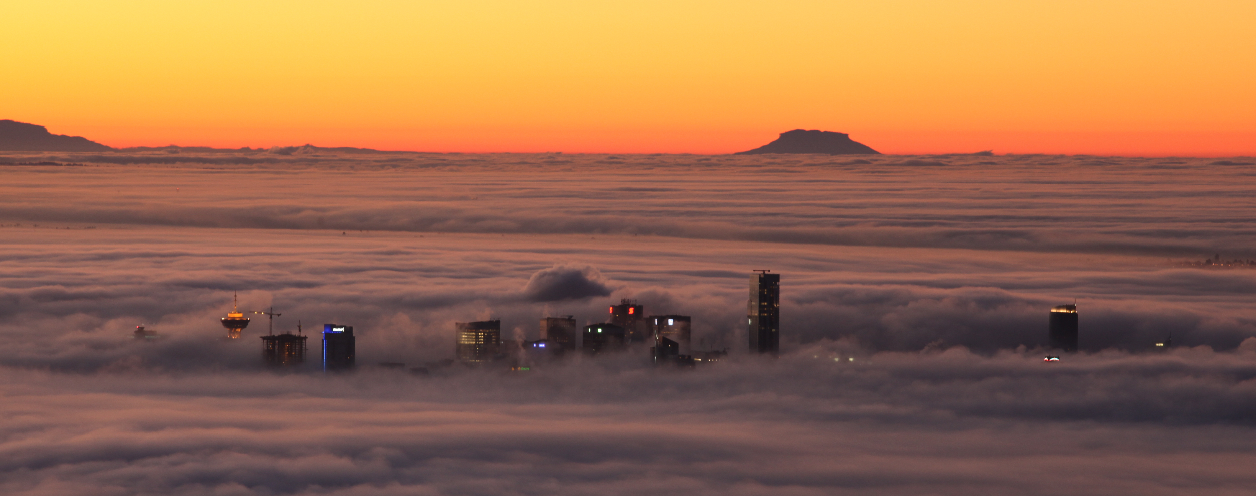
\includegraphics[width=\linewidth]{CypressView}
%  \caption{%
%  	In the Clouds: Vancouver from Cypress Mountain.
%  	Note that the teaser may not be wider than the abstract block.%
%  }
%  \label{fig:teaser}
%}

%% Uncomment below to disable the manuscript note
%\renewcommand{\manuscriptnotetxt}{}

%% Copyright space is enabled by default as required by guidelines.
%% It is disabled by the 'review' option or via the following command:
%\nocopyrightspace


%%%%%%%%%%%%%%%%%%%%%%%%%%%%%%%%%%%%%%%%%%%%%%%%%%%%%%%%%%%%%%%%
%%%%%%%%%%%%%%%%%%%%%% LOAD PACKAGES %%%%%%%%%%%%%%%%%%%%%%%%%%%
%%%%%%%%%%%%%%%%%%%%%%%%%%%%%%%%%%%%%%%%%%%%%%%%%%%%%%%%%%%%%%%%

%% Tell graphicx where to find files for figures when calling \includegraphics.
%% Note that due to the \DeclareGraphicsExtensions{} call it is no longer necessary
%% to provide the the path and extension of a graphics file:
%% 
\includegraphics{diamondrule} is completely sufficient.
\graphicspath{{figs/}{figures/}{pictures/}{images/}{./}} % where to search for the images

%% Only used in the template examples. You can remove these lines.
\usepackage{tabu}                      % only used for the table example
\usepackage{booktabs}                  % only used for the table example
\usepackage{lipsum}                    % used to generate placeholder text
\usepackage{mwe}                       % used to generate placeholder figures

%\usepackage{tikz,lipsum,lmodern}
%\usepackage[most]{tcolorbox}
%\usepackage[bookmarksnumbered,unicode]{hyperref}
%% We encourage the use of mathptmx for consistent usage of times font
%% throughout the proceedings. However, if you encounter conflicts
%% with other math-related packages, you may want to disable it.
\usepackage{mathptmx}                  % use matching math font

%Setups

\newcommand{\gaia}{{\textsc{Gaia}}}

\newcommand{\eg}{{\it e.g.,\ }}
\newcommand{\etal}{{\it et al.\ }}
\newcommand{\etc}{{\it etc.}~}
\newcommand{\etcns}{{\it etc.}}
\newcommand{\ie}{{\it i.e.,\ }}

% \definecolor{bluecrayola}{rgb}{0.12,0.46,1.0}
% \newcommand{\revise}[1]{{\color{bluecrayola} #1}}
% \newcommand{\review}[1]{\textcolor{purple}{[#1] }}

%\definecolor{bluecrayola}{rgb}{0.12,0.46,1.0}
\newcommand{\todo}[1]{{\color{bluecrayola} #1}}

% keywards
\newcommand{\aniclass}{{\textit{AniClass}}}
\newcommand{\aniunit}{{\textit{AniUnit}}}
\newcommand{\code}[1]{{\texttt{#1}}}


\newcommand{\squishlist}{
	\begin{list}{$\bullet$}
		{ \setlength{\itemsep}{0pt}
			\setlength{\parsep}{1pt}
			\setlength{\topsep}{1pt}
			\setlength{\partopsep}{0pt}
			\setlength{\leftmargin}{1.6em}
			\setlength{\labelwidth}{1em}
			\setlength{\labelsep}{0.6em}
		}
	}
	\newcommand{\squishend}{
	\end{list}
}


\begin{document}

%%%%%%%%%%%%%%%%%%%%%%%%%%%%%%%%%%%%%%%%%%%%%%%%%%%%%%%%%%%%%%%%
%%%%%%%%%%%%%%%%%%%%%% START OF THE PAPER %%%%%%%%%%%%%%%%%%%%%%
%%%%%%%%%%%%%%%%%%%%%%%%%%%%%%%%%%%%%%%%%%%%%%%%%%%%%%%%%%%%%%%%

%% The ``\maketitle'' command must be the first command after the
%% ``\begin{document}'' command. It prepares and prints the title block.
%% the only exception to this rule is the \firstsection command
%\firstsection{Introduction}

\maketitle


\section{Introduction}
\label{sec:intro}

%% infographics is useful
%Infographics use a combination of graphics, text, images, and data to inform and engage.
%In animated infographics, some elements are animated to illustrate data or emphasize key points more excitingly and engagingly.
%% animated infographics are useful
Animated infographics is considered a powerful tool for storytelling. 
It has been widely used in multiple areas, such as business, publicity, science popularization and so on. 
Compared to static infographics, it can interpret data or ideas more vividly and grabs the audience's attention quickly, appreciated and shared by people for years~\cite{blazer2019animated, brehmer2016timelines}. % [5, 10] in "Communicating with Motion: A Design Space for Animated Visual Narratives in Data Videos"

% introduce existing approaches and shortcomes
%Unfortunately, the creation of animated infographics is tedious and time-consuming, especially for novice users~\cite{amini2016authoring, hullman2013deeper, shi2021communicating}. %[5 dataclip, 41, 80, in Katika]
%It can take weeks to authorize graphical animation itself that lasts around one minute \cite{howlong}.
%\qmhl{Creating animated inforgraphics from scratch involve two major steps: static inforgraphics designing and animation creating~\cite{jahanlou2020challenges, shi2021communicating}.}
%Initially, designers need to create static infographics (like te rightmost figure in \autoref{fig:ani_example}(A)) using feature-rich software such as Adobe Illustrator~\cite{AdobeAI} and  export them as Scalable Vector Graphics (SVGs) or other kinds of files so that downstream tools can be employed for animation creation.
%Then, the interactive tools (\eg Adobe After Effects~\cite{AdobeAE}) are used to add animations.
%However, they only provide low-level operations, like keyframes or interpolation, for motion authoring, which requires expertise and is time-consuming \cite{jahanlou2020challenges}.
%Some users might choose programming tools (\eg D3~\cite{bostock2011d3}) because they can precisely control property changes and organize timelines through program flow.
%In recent years, declarative languages are preferred by designers for this task as they favor conciseness over expressiveness~\cite{mcnutt2023nogrammar}. 
%Canis~\cite{ge2020canis} falls into this category, which provides a declarative language for creating animated charts.
%These techniques simplify the creation process but can only use a predefined library of simple animations usually, which limits their usage.
%Here, we introduce two examples to better illustrate the challenges of creating animated infographics with existing tools.

Crafting animated infographics is tedious and time-consuming, particularly for novice users~\cite{amini2016authoring, hullman2013deeper, shi2021communicating}. The process to produce just one minute of graphical animation can span several weeks \cite{howlong}.
The construction of animated infographics fundamentally comprises two primary stages: designing static infographics and creating animation~\cite{jahanlou2020challenges, shi2021communicating}. Initially, designers employ feature-rich software like Adobe Illustrator~\cite{AdobeAI} to craft static infographics (as exemplified by the rightmost figure in \autoref{fig:ani_example}(A)). Subsequently, these are exported as Scalable Vector Graphics (SVGs) or other file types to leverage downstream tools for animation. 
In the following stage, interactive tools such as Adobe After Effects~\cite{AdobeAE} are utilized to create animations. However, these tools only offer low-level operations like keyframes or interpolation for motion authoring, which requires a significant degree of expertise and time \cite{jahanlou2020challenges}. 
%\qmpr{ Some designers might gravitate towards programming tools like D3~\cite{bostock2011d3} for the precision they offer in controlling property changes and organizing timelines through program flow.}{What's the benefits and disadvantage of D3?}
In recent years, designers have shown a preference for declarative languages due to their succinctness, even if it sometimes comes at the cost of expressiveness \cite{mcnutt2023nogrammar}. Canis \cite{ge2020canis} falls into this category, offering a declarative language tailored for crafting animated charts. 
%\qmpr{These techniques simplify the creation process but can only use a predefined library of simple animations usually, which limits their usage}{Failed to clearly introduce the limitation of Canis}.
%\qmhl{Here, we introduce two examples to better illustrate the challenges of creating animated infographics with existing tools.}
\qmhl{However, these methods are either designed for data-driven chats or lack flexibility for reuse across diverse infographics}

% Examples

\begin{figure*}[h]
  \centering
  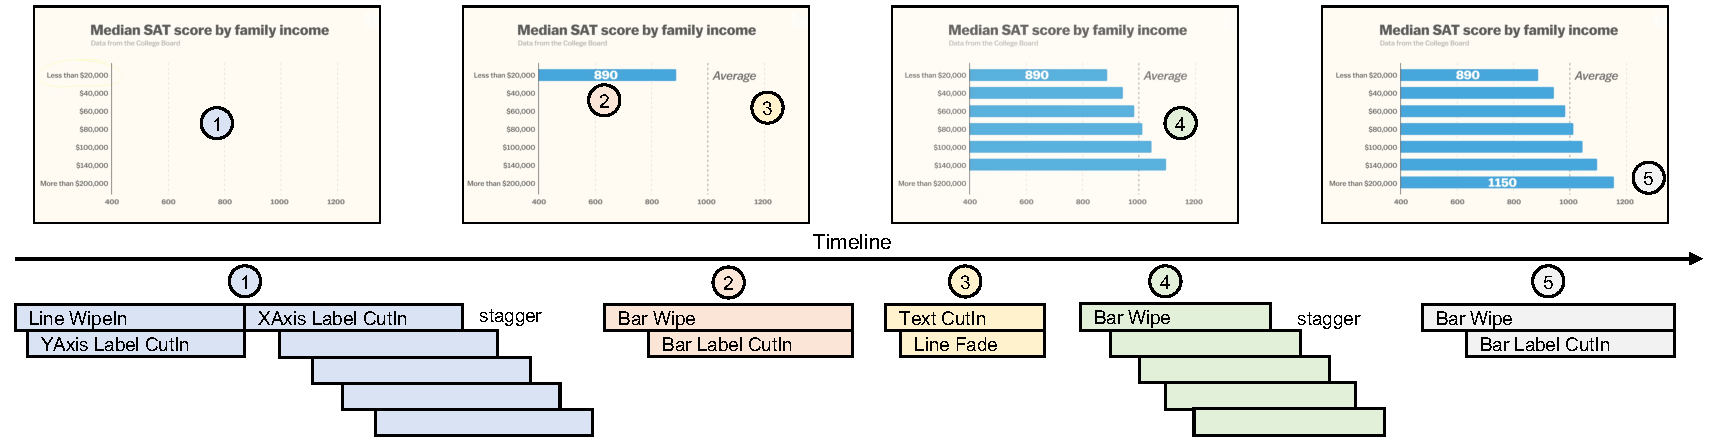
\includegraphics[width=\linewidth]{figs/ani_example_tvcg.pdf}
  \caption{An animated infographic about the correlation between SAT score and family income which are retrieved from \url{https://youtu.be/WjVVwMGJ9S8?t=334}.}
%  \Description{(A) An animated infographic about the pretrial released defendants of the D.C. court in 2017. (B) An animated infographic about the relation between SAT score and family income. Similar animations are framed in blue.}
  \label{fig:ani_example}
\end{figure*}

%\autoref{fig:ani_example}(A) illustrates four keyframes and the timeline of an animated.
%The creation process is as follows:
%% A1
%To implement the CutIn effect in A1, each element needs to be masked separately.
%In A1, the y coordinates of title texts should be set at the start/end keyframe to let them move out from the masks.
%% A2-3
%Then following the narration, three similar animation groups are created at the corresponding timestamp (A2-4).
%In each group, the bar enters using a Wipe effect (the mask is also required) and texts of the axis and the bar enter using CutIn.
%The relative offsets, durations and easing functions for each animation are carefully set to produce a harmonious result.

An example is shown in \autoref{fig:ani_example}. 
Given a static SVG, five animations (\circled{1}-\circled{5}) are added.
First, the chart framework enters at the beginning when the author explains this chart (shown as \circled{1}) .
Each element's animation is individually managed, employing varying effects tailored to the specific element.
For example, the lines use the WipeIn effect, while the x-label on the left uses the CutIn effect. 
Increasing offsets are set for the x-axis labels to achieve the stagger effect.
Following the narration, the bar and bar label for the category ``less than \$20,000'' enter (shown as \circled{2}).
A line and a label fade in to illustrate the average score (shown as \circled{3}).
Then, bars in the middle wipe in with a stagger (shown as \circled{4}) to show a positive correlation.
Finally, the corresponding bar and label for ``More than \$200,000'' are animated with similar effects (shown as \circled{5}).

% Obstacles

Two obstacles hinder the designer's creation process. 
First, \textbf{non-intuitive and expert-driven creation approaches}. % [34, 44] in katika?
During the creation, each animation needs to: 
1) select one animation target;
2) create a start keyframe at the appropriate timestamp and set initial properties;
3) create an end keyframe at the appropriate timestamp and set final properties;
4) specify an appropriate easing function.
Designers need to deal with these cumbersome settings with an understanding of underlying concepts like keyframes, channels, \etc~\cite{krasner2013motion, sarinastiti2016skill}
This is labor-intensive but unavoidable even for experts \cite{jahanlou2020challenges}.
Second, \textbf{the repetitive creation of animations}.
We observe that animations share similarities, not only between different element groups of the same instance but also across multiple similar instances.
For example, animations framed in blue in \autoref{fig:ani_example} are similar and applied on the bars and bar labels, which can be extracted and reused.
As another example, entering animations of axes exist in many animated chart videos.
As mentioned by Thompson \etal~\cite{thompson2020understanding}, reusing animations on similar groups is useful, which simplifies and speeds up the creation process.
% conclusion
Given these situations, though these existing tools are helpful, designers of animated infographics still take a procedural approach to create them from scratch: draw the elements, select targets and create animations one by one.
% as mentioned in the work of Thompson \etal~\cite{thompson2020understanding}.
% Besides, specifying visual properties is not an intuitive way for animation creation and requires expertise~\cite{}.

% Gaia
In this work, we aim to reduce the burden of creating animated infographics greatly. 
We propose \gaia{}, a declarative \underline{\textsc{G}}rammar for \underline{\textsc{a}}nimated \underline{\textsc{i}}nfogr\underline{\textsc{a}}phics. 
\gaia{} is motivated by three goals.

\textbf{Expressivity}: \gaia{} is both expressive and intuitive for reading and writing.
In \gaia{}, animations are represented by effects applied to a group of visual elements instead of keyframes created individually for each separate element.
% insight: hierarchy of groups and animations
Groups in one infographic (as we called, instance) form a hierarchy and each group can apply effects.
Besides, grouping is also a way to organize animations~\cite{thompson2020understanding}. Animations for groups can be combined with several alignment strategies (\eg start before previous), which also form a hierarchical structure simplifying the creation and refinement of timelines. 
% Gaia
\gaia{} provides a declarative grammar following these insights, which enables designers to create animations for groups and organize them in a hierarchical timeline.
In this way, \gaia{} can support flexible and intuitive animation creation for infographics and enable users to express and refine complex animation timelines easily.
% Meanwhile, a wider variety of groups of different elements can also be animated using \gaia{}.

\textbf{Reusability}: Animations in \gaia{} can be reused.
% insight: animations share similarity
As mentioned above, reusing similar animations saves time and effort \cite{jahanlou2022katika}.
However, due to the diversity of animated objects, it is challenging even for a single simple animation, let alone a well-designed animation combo.
% Gaia
In \gaia{}, animations are declared for a class of infographics, not a concrete instance.
To this end, we conduct a target abstraction to describe graphical elements in infographics.
The animations are not directly bound to the graphical elements but instead, bound to the role of the elements in a unified representation.
For example, \gaia{} can declare a design for different types of animated elements in axes, such as domain, ticks and labels, without relying on a concrete instance.
A wide range of SVGs from the internet or other design tools can be transformed into a format that contains the roles of each animated target and other information (like data). 
Then users can reuse complex but well-designed animations from themselves or other designers.

\textbf{Extensibility}: Template library in \gaia{} can be extended.
% insight
Good design (including the coordination of effects, the design of parameters, \etcns) is difficult to express, store, and share in multiple creations.
% This is because developers are usually not professional animators.
Some existing declarative languages provide an animation library, but provided effects are preset and simple, like fade and wipe, designed for generic usage.
Meanwhile, these techniques don't provide support for extending the animation library. The only way to do this is through a code-level implementation.
% Gaia
Based on the target abstraction, \gaia{} allows expert designers to define new templates easily through a consistent declarative grammar as animation creation, then register them to the library and all users can use them just as other existing templates. 
For example, users can combine templates for bars and axes to create a new template for bar charts. 
Parameter abstraction is also introduced in \gaia{} so that a template can be more generic and customizable.

We implemented a \gaia{} compiler and released it as a TS library, which can be embedded in other tools as an animation engine with high-level specs as input.
Through a demo system with a variety of examples, we show the expressive of \gaia{}.
We conducted a user study with 8 participants with no animation design experience to illustrate the ease of use of \gaia{} and gather feedback.
All participants can acquire the core features of \gaia{} within 1h of learning, and successfully replicate the data video designed by professionals.
\gaia{} has been applied in a real-world project, and through interviews with three experts who employed it extensively, we garnered positive feedback and valuable suggestions for future improvements.

In brief, the main contributions of this work, in presentation order, include:
% \begin{enumerate}
% \item \textbf{A set of high-level grammars} that enables intuitive creation of animations (\autoref{sec:gaia_ani}). 
% Users can build complex animations via a hierarchical view and concatenating operations. 
% \item \textbf{Target abstraction} decouples animation declarations from concrete instances, enabling reusability and extendability of \gaia{}, which is the first attempt for declarative animation grammars (\autoref{sec:gaia_reuse}).
% \item \textbf{A compiler prototype} and \textbf{workflow} of \gaia{} in different points of views (\autoref{sec:workflow}).
% \item \textbf{An evaluation} on the usability of \gaia{}, including \textbf{a demo system} with multiple examples used in case studies and a user study involved both novice users and experts in animation design (\autoref{sec:eval}).
% \end{enumerate}

\squishlist 
\item \textbf{A set of high-level grammars} that enables intuitive creation of animations (\autoref{sec:gaia_ani}). 
Users can build complex animations via a hierarchical view and concatenating operations. 
\item \textbf{Target abstraction} decouples animation declarations from concrete instances, enabling reusability and extendability of \gaia{}, which is the first attempt for declarative animation grammars (\autoref{sec:gaia_reuse}).
\item \textbf{A compiler prototype}\footnote{The src code and the deployment version of both \gaia{} compiler and demo system are available in supplementary materials. An online version of the demo system is also available at \url{https://gaia-ui.azurewebsites.net}.} and \textbf{workflow} of \gaia{} in different points of views (\autoref{sec:workflow}).
\item \textbf{An evaluation} on the usability of \gaia{}, including \textbf{a demo system} with a variety of examples used in the case study, a user study involved novice users, and semi-structured interviews conducted with experts experienced in using \gaia{}.
\squishend
\section{Related Work}

In this section, we discuss previous work related to \gaia{} from 3 aspects: infographic and animation for infographics, visual animation authoring tools and programming approaches for animation authoring.

\subsection{Infographic and Animation for Infographics}
% infographics
The number of work on infographics published in recent years has increased.
Infographics combine a variety of data-encoded elements and embellishments, which can attract readers’ interests easily~\cite{bateman2010useful, haroz2015isotype, borkin2013makes, wang2019emotional}. % from InfoMotion [BMG∗10, HKF15, BVB∗13, WSK∗19]
% hierarchy; Visual Information Organization
Some existing researches attempt to understand infographics from semantic meanings of visual elements~\cite{lu2020exploring, wang2021animated}. 
Lu \etal~\cite{lu2020exploring} gave a concept of visual information flow. They pointed out one infographic can contain multiple visual groups that share similarity. 
These groups are laid out to follow a backbone and form a hierarchy of infographics naturally.
Wang's work~\cite{wang2021animated} also illustrated this insight existed in a large range of real infographics.
They named such groups as repeating units and pointed out that different visual elements in a group can have different roles semantically.
% nested hierarchy
Nested structure in the element hierarchy is common and can be easily created via some DSLs like D3~\cite{bostock2011d3} and Protovis~\cite{heer2010declarative}.
In the work of Liu \etal~\cite{liu2018data}, visual elements are arranged by collections, which can be nested for organization.
For example, some infographics contain several stacked bars, which form a multi-layered hierarchy: stacked bar groups and rectangles in each group.
% relation to Gaia
In \gaia{}, we follow the intuition of nested hierarchy in infographics to build an abstraction of animated targets. 

% animated infographics
Animated infographics are regarded as an efficient tool that can express an informative story using intuitive and attractive effects applied on visual elements~\cite{blazer2019animated, brehmer2016timelines}.
Researchers have investigated a wide range of cases from the real world and conducted surveys for understanding and creation~\cite{wang2021animated, shi2021communicating}. 
% InfoMotion
By collecting animations of infographics from multiple sources, like PowerPoint templates and video sites, Wang \etal~\cite{wang2021animated} summarized the design space of animated infographics. 
They claimed that effects can be applied to a group of elements, then be organized via three arrangement styles.
\gaia{} borrows the primitives of timing arrangement and adapts them to animations with a more complex timeline.
% Nan's survey
Some other work focus on effects used in animations~\cite{shi2021communicating}.
They derived animated visual narratives that fall into 8 categories of narrative strategies. 
These work inspire the design of animations in \gaia{}, but with the type system, \gaia{} can design animations for a semantic group of elements by combining these primitive effects.

\subsection{Visual Animation Authoring Tools}

Creation of animated infographics is a challenging task~\cite{jahanlou2022katika, howlong}, so a few visual animation authoring tools are proposed.
% Keyframe-based tools
Keyframe-based tools, like Adobe After Effects~\cite{AdobeAE} and Data Animator~\cite{thompson2021data}, provided low-level operations for motion creation.
They allow users to specify the properties of visual elements on each keyframe and create intermediate frames according to the easing function.
Besides, it is time-consuming when creating or modifying visual properties and time settings on a set of marks.
\gaia{} doesn't need to define keyframes. Instead, high-level grammar is employed for easy reading and writing.

% Template-based
Template-based tools, as another category, provide a set of preset templates to facilitate animation creation.
PPT~\cite{msppt}, DataClips~\cite{amini2016authoring} and Flourish~\cite{flourish} fall into this category.
In these tools, animations can be created intuitively and easily by applying templates on targeted elements instead of adjusting low-level properties. 
However, most of them only provide a small number of effects and can't be extended, which limits their applicability. 
Besides, their flexibility relies on pre-defined templates, thus are less expressive.
As such, creating complex animations with them is difficult, even impossible.
Data Player~\cite{shen2023dataplayer} interweaves data video authoring with narrations, providing a set of pre-designed animation presets.
Katika~\cite{jahanlou2022katika} provides an end-to-end solution for creating animated graphics visually and also provides a motion library that can be extended by the community. 
Although it simplifies the creation pipeline, Katika can only employ statics graphics (called artworks in Katika) from its own embedded library.
% Gaia
\gaia{} also uses a concept of templates and allows users to extend them smoothly.
As a high-level grammar, \gaia{} and its compiler can be integrated as a part of interactive tools for animated infographics authoring.
We refer interested readers to the survey on visualization authoring methods conducted by Grammel \etal~\cite{grammel2013survey}.

\subsection{Programming Approaches for Animation Authoring}
To create animation more accurately and easily, some designers prefer programming approaches, which can be categorized into low- and high-level languages.
% low-level
Low-level languages, such as processing~\cite{processing} and D3~\cite{bostock2011d3}, provide APIs for low-level operations that enable users to control the properties of animated targets directly.
For example, D3 uses a transition operation that enables users to indicate what and how visual properties (\eg width and color) change on selected elements.
Due to their high expressiveness, these languages have gained widespread use for creating custom and informative animations.
However, they require users to have experience in graphic editions and animation creation, resulting in a steep learning curve. 
Users need to specify when and how these properties change for every element in detail, which is non-intuitive and time-consuming for complex animations with many animated elements.

% high-level
High-level languages are typically preferred as they favor conciseness over expressiveness~\cite{mcnutt2023nogrammar}. 
% json-based
Some languages adopt JSON to express animations at a high level~\cite{zong2022animated, kim2020gemini, kim2021gemini, ge2020canis, ge2020canis, ge2021cast}. %[Animated Vega-Lite, Gemini, Gemini2, Canis, CAST, Lottie]
Gemini and Gemini2~\cite{kim2020gemini, kim2021gemini} focus on transitions between two static visualizations. 
Animated Vega-Lite~\cite{zong2022animated} is proposed for generating animations and binding logic for interactive graphics. 
% hiding complexity
With hiding under-layered mechanisms, some grammars describe animations as effects applied on selected elements, thus are more intuitive and concise compared to the low-level languages.
For example, Canis and CAST~\cite{ge2020canis, ge2021cast} provide several basic pre-defined effects to create animation without setting the initial and end values of properties.
Via grouping operation, they can bind effects to a set of marks with a given align strategy thus the number of animations defined can be reduced.
While these languages create satisfied animations quickly with concise specifications, they focus on data-driven charts instead of infographics.
Another language, gganimate~\cite{gganimate}, uses concise code to express animations.
Similar to Canis, it also employs encapsulation of animations to hide the details.
However, it is mainly designed to create transitions for a specific chart type and can only be used in the programming language R.

% Gaia
Inspired by these work, \gaia{} is designed with a JSON-style grammar that strikes a good balance between expressiveness and conciseness.
% first difference
\gaia{} is the first one who considers types in animation authoring.
According to our insights, elements in an infographic have different types and form a hierarchy. 
Exiting methods, like Canis, can only process groups of the same marks.
Without awareness of types of animated targets, high-level languages can only provide generic and simple effects (such as fade and wipe in Canis, enter\_fade in gganimate), which makes spec verbose when creating complex animations.
% second difference
% Besides, pre-defined effects set in both Canis and gganimate are hard to extend.
Besides, pre-defined effect sets of existing tools are hard to extend.
McNutt~\cite{mcnutt2023nogrammar} pointed out the value of extensibility in DSLs, but none have provided a satisfactory solution for it in the field of animation creation.
\gaia{} brings extensibility to this kind of grammar for the first time to create new animations or target types in a declarative way and enable reusing, which facilitates creation greatly.
% \section{Motivation and Design Considerations}
\label{sec:motivation}

% [18, 55] katika crowdsourcing community-based approaches

\gaia{} is a high-level declarative language that enables rapid specification of animated infographics.
Taking a static SVG as input, \gaia{} compiler generates a playable animated infographics instance according to the \gaia{} specification.
As mentioned in \autoref{sec:intro}, \gaia{} is designed to be expressive, reusable, and extensible.
Inspired by Katita~\cite{jahanlou2022katika}, animations in \gaia{} are also treated as \textit{independent entity} and can be reused in one instance or across different instances (\ie artworks in Katika).
Following the design of Gemini~\cite{kim2020gemini} and Canis~\cite{ge2020canis}, \gaia{} \textbf{manage animations in a hierarchical structure}, providing constraints that describe the relationship between animations.

Such an animation structure allows some composite animation designs (\eg the animation of ) to be reused within a single instance, but not between different instances.
Because the internal structure and elements of infographics vary from instance to instance.
Unlike some interactive tools (\eg Katika), the input SVG of \gaia{} can be created by any upstream tools (like D3~\cite{bostock2011d3}, Vega-Lite~\cite{satyanarayan2016vega}, Adobe Illustrator ~\cite{AdobeAI}, \etcns).
Canis provides a possible solution to bind roles to elements: set ids, classes, and data to SVG elements and generate dSVG.

This motivates us to design a \textbf{tree-like target abstraction} for \gaia{}.


Then unstructured SVGs need to be mapped to the target abstraction to enable reusability.

To sum up, 

\section{The \gaia{} Grammar of Animation}
\label{sec:gaia_ani}

%\gaia{} is a high-level declarative language that enables rapid specification of animated infographics.
%Taking one static SVG as input, \gaia{} compiler generates a playable animated infographic instance according to the \gaia{} specification.
%In this section, we introduce the \gaia{} grammar \qmhl{with an simple example shown as \autoref{fig:ani_spec} (A).} 
%This example demonstrate an animation of four elements: two values (40 and 50) and two bars indicating these two values with their height. The animation of this graphics is indicated by \autoref{fig:ani_spec} (B). The whole animation last fore 1.5 seconds shown as the first line. The bars extend vertically along the whole time range. The number shown on the top of the bars appears as a zoom manner during the time range betweewn 0.5s to 1.5s.
%
%\gaia{} is a high-level declarative language that enables rapid specification of animated infographics.
%Taking one static SVG as input, \gaia{} compiler generates a playable animated infographic instance according to the \gaia{} specification.
%In this section, we introduce the \gaia{} grammar \qmhl{with an simple example shown as \autoref{fig:ani_spec} (A).} 
%This example demonstrate an animation of four elements: two values (40 and 50) and two bars indicating these two values with their height. The animation of this graphics is indicated by \autoref{fig:ani_spec} (B). The whole animation last fore 1.5 seconds shown as the first line. The bars extend vertically along the whole time range. The number shown on the top of the bars appears as a zoom manner during the time range betweewn 0.5s to 1.5s.

\gaia{} is a high-level declarative language designed for the rapid creation of animated infographics. 
Given a static SVG as input, the \gaia{} compiler produces an animated infographic based on the \gaia{} specifications. 
In this section, we present the grammar of \gaia{}, illustrated with a straightforward example in \autoref{fig:ani_spec} (A). 
This example showcases an animation of four elements: two numerical values (40 and 50) and two bars that represent these values by their height. 
The animation sequence can be observed in \autoref{fig:ani_spec} (B). 
The entire animation spans 1.5 seconds, as indicated in the first line in \autoref{fig:ani_spec} (B). 
Throughout this whole duration, the bars extend vertically. 
The numbers shown on the bars are appeared through a zooming effect between 0.5s and 1.5s.






\subsection{Animation Specification}
\label{ssec:aniclass_aniunit}

%A \gaia{} animation spec (as we called \aniclass{}) describes the animation applied on a given infographic with several animation units (as we called \aniunit{}) and a set of setting attributes.
%\autoref{fig:ani_spec}(A) shows an example of animation spec.
%It contains 3 \aniunit{}s: Sync animation, Wipe animation of bars, and ZoomIn animation of the bar labels.
%The animation created and the corresponding timeline are shown in \autoref{fig:ani_spec}(B).
%To ease understanding, each attribute is associated with an attribute type given in \autoref{fig:ani_spec}(C).
%Attribute \code{main} (line 5-19) defines the body of this animation, which contains a single \aniunit{}.
%Other attributes of type \textit{Class} (line 2-4) address the reusability of \gaia{}, which will be discussed in \autoref{ssec:extend_template}.

%A \gaia{} animation spec (as we called \aniclass{}) describes the animation applied on a given infographic with several animation units (as we called \aniunit{}) and a set of setting attributes.
%\autoref{fig:ani_spec}(A) shows an example of animation spec.
%It contains 3 \aniunit{}s: Sync animation, Wipe animation of bars, and ZoomIn animation of the bar labels.
%The animation created and the corresponding timeline are shown in \autoref{fig:ani_spec}(B).
%To ease understanding, each attribute is associated with an attribute type given in \autoref{fig:ani_spec}(C).
%Attribute \code{main} (line 5-19) defines the body of this animation, which contains a single \aniunit{}.
%Other attributes of type \textit{Class} (line 2-4) address the reusability of \gaia{}, which will be discussed in \autoref{ssec:extend_template}.


Given an infographic (using SVG as an example), \gaia{} employs \aniclass{} to dictate the animation of its visual elements. An \aniclass{} is composed of several setting attributes and animation units, termed as \aniunit{}s within Gaia. A detailed exposition of these setting attributes can be found in \autoref{tab:setting}. 
These attributes outline the foundational information for animation specification. Users have the flexibility to explicitly incorporate libraries and their custom animations using the "package" and "import" attributes, respectively. Animation configurations can be defined via the "name," "targetType," and "params" attributes. Furthermore, the "main" attribute signifies the starting point of the animation.


%\autoref{fig:ani_spec}(A) shows an example of animation spec.
%It contains 3 \aniunit{}s: Sync animation, Wipe animation of bars, and ZoomIn animation of the bar labels.
%The animation created and the corresponding timeline are shown in \autoref{fig:ani_spec}(B).
%To ease understanding, each attribute is associated with an attribute type given in \autoref{fig:ani_spec}(C).
%Attribute \code{main} (line 5-19) defines the body of this animation, which contains a single \aniunit{}.
%Other attributes of type \textit{Class} (line 2-4) address the reusability of \gaia{}, which will be discussed in \autoref{ssec:extend_template}.

The example shown in \autoref{ssec:extend_template}. The ``main'' attributes (line 5-19) defines the body of this animation, which is a single \aniunit{} ``sync''. There are another two \aniunit{}s are defined into ``sync'' which are the Wipe animation of bars and the ZoomIn animation of labels.

\begin{figure}[h]
  \centering
  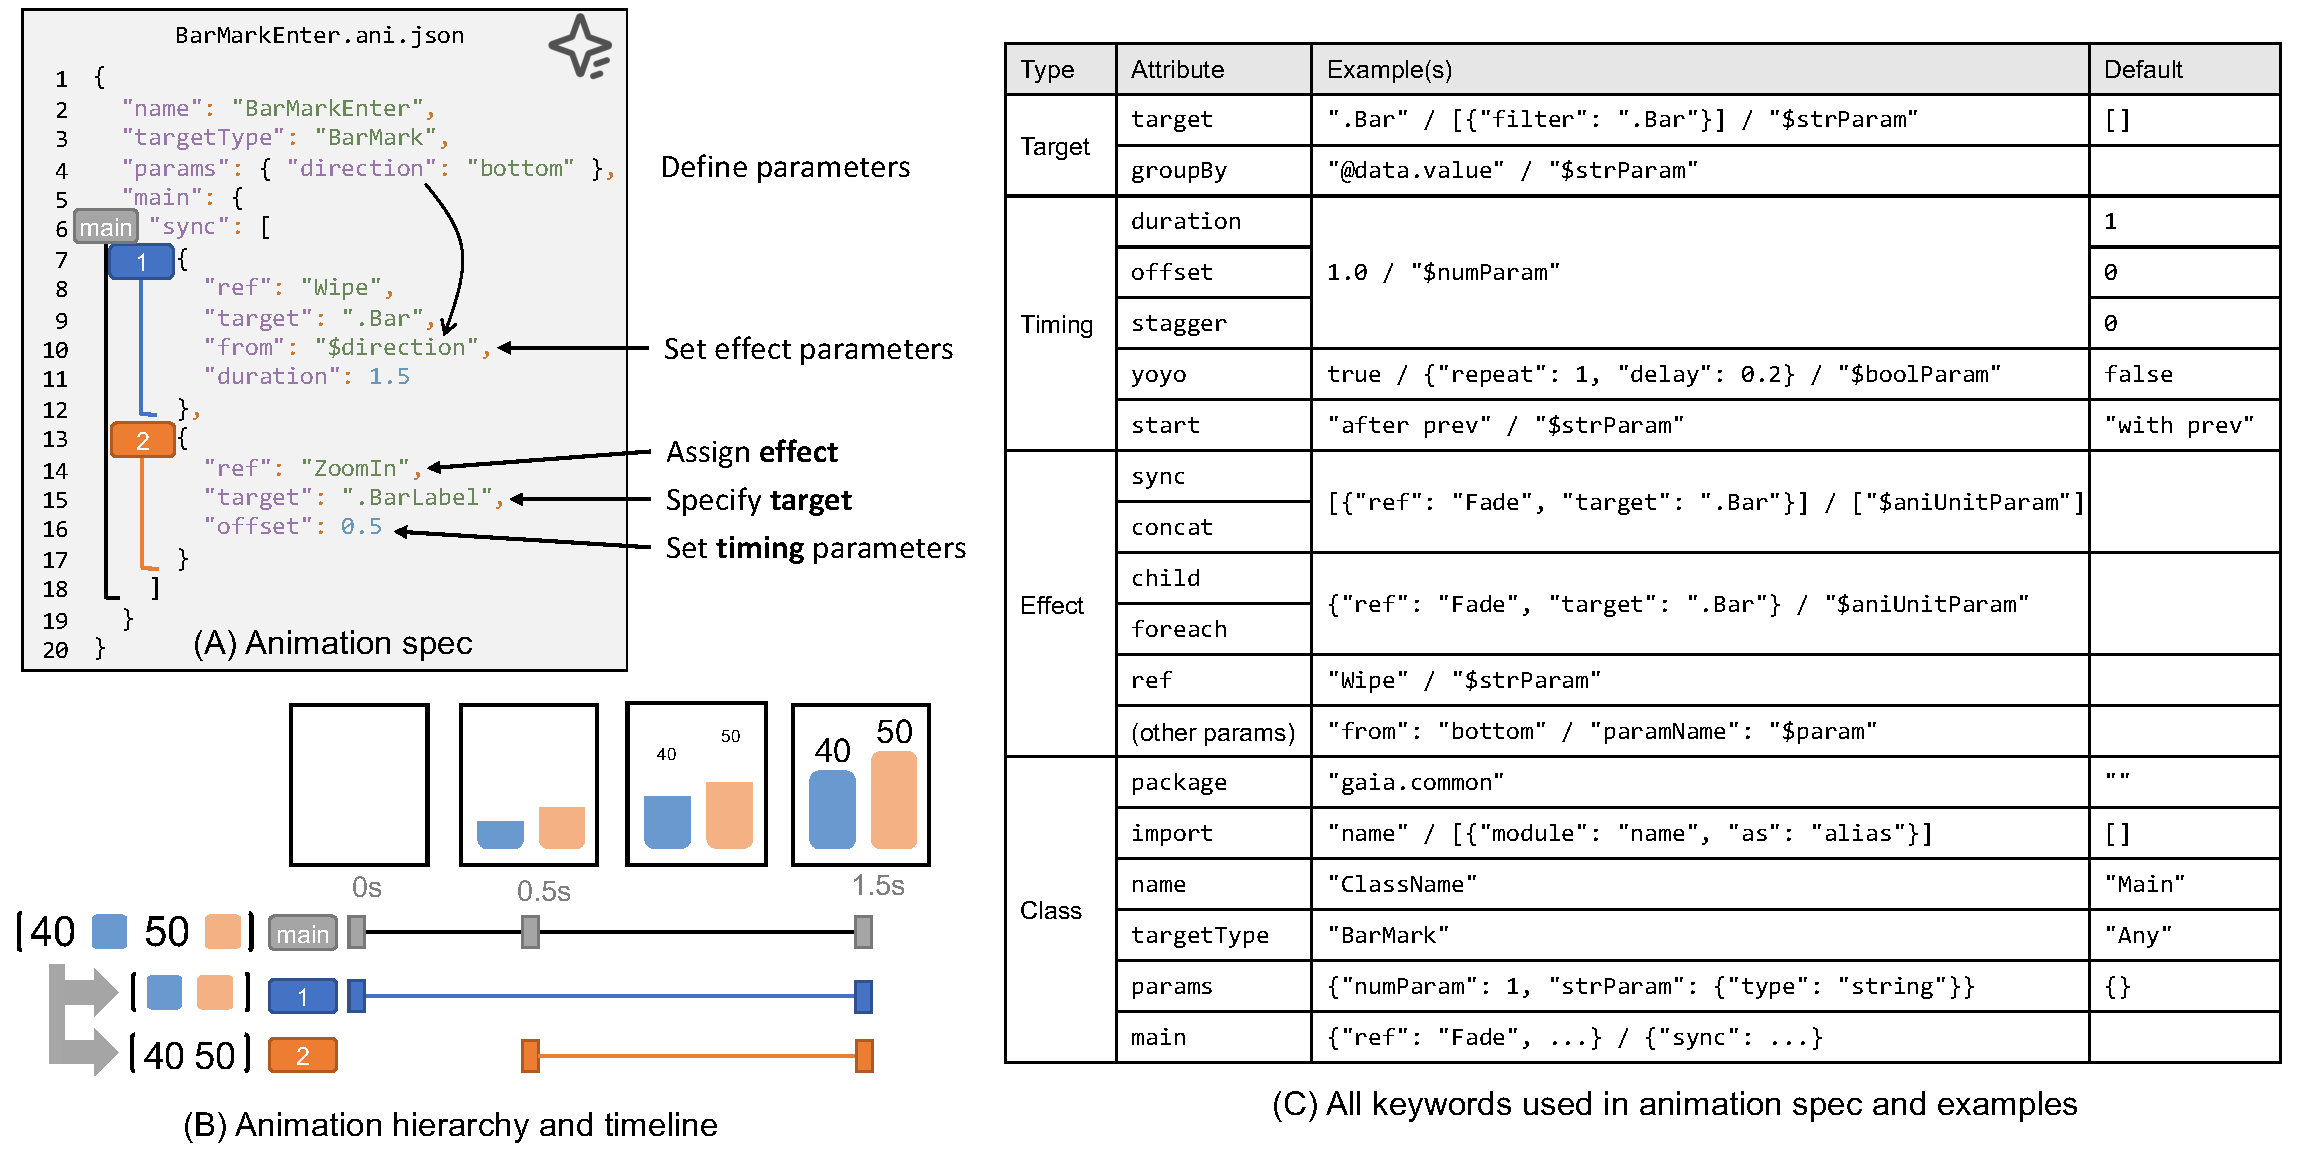
\includegraphics[width=\linewidth]{figs/ani_spec.pdf}
  \caption{
  (A) An example of \gaia{} animation spec, \ie \aniclass{}, designed for BarMark. It contains 3 \aniunit{}s. 
  (B) An animated instance and timeline of the animation created by this spec. \aniunit{}s form a tree hierarchy and each animation selects targets from the parent. 
  (C) All keywords used in \gaia{} animation spec and examples. }
%  \Description{(A) An example of \gaia{} animation spec, \ie \aniclass{}, designed for BarMark. It contains 3 \aniunit{}s. 
%  (B) An animated instance and timeline of the animation created by this spec. \aniunit{}s form a tree hierarchy and each animation selects targets from the parent. 
%  (C) All keywords used in \gaia{} animation spec and examples. }
  \label{fig:ani_spec}
\end{figure}

\aniunit{} describes the effects (using \code{ref}) applied on groups of elements (specifying by \code{target}). 
Formally, one \aniunit{} is an object that contains three types of attributes:
$$
AniUnit := \langle Target, Timing, Effect \rangle
$$
\textit{Target} (\autoref{ssec:gaia_ani_target}) declares the animated target.
Attribute \code{target} defines a list of transforms specifying how an \aniunit{} picks and reshapes targets from its parent.
Attribute \code{groupBy} can only be used with \code{foreach} (introduced in \autoref{ssec:gaia_ani_effect}), grouping the selected elements and applying the effect to each group.
\textit{Timing} (\autoref{ssec:gaia_ani_timing}) contains 4 attributes that describe the common timing settings of an animation.
Attributes of type \textit{Effect} (\autoref{ssec:gaia_ani_effect}) describe how to perform the animation.
One \aniunit{} can refer to an existing effect using \code{ref} (like line 8, 14 in \autoref{fig:ani_spec}(A)).
Especially, \aniunit{} can be nested, using attributes \code{sync}/\code{concat}/\code{foreach}/\code{child} to combine child \aniunit{}s (like \code{sync} animation in \autoref{fig:ani_spec}(A)).
Other animation-related parameters also fall into this category.
\autoref{fig:ani_spec}(C) gives a full list of the attributes and provides some examples.
Strings started with symbol \code{\$} are placeholders for parameters, which will be discussed in \autoref{sec:gaia_reuse}.


\subsection{Target and Target Selection}
\label{ssec:gaia_ani_target}

% Target attribute declared the animated target of \aniunit{}s. 
% Before introducing how target selection works in \gaia{}, we need to formulate the data structure of animated targets.
% As explained by Liu \etal~\cite{liu2018data}, the concept of a collection is defined as a list of elements of the same type, whereas a group can comprise elements of different types.
% Following by the idea of scene graph in Satyanarayan \etal's work~\cite{satyanarayan2015reactive}, \gaia{} abstracts the animated target as a \textbf{tree structure} where leaf nodes are atomic visual elements and internal nodes are groups.
% This abstraction is similar to the SVG structure utilizing \code{g} elements, as shown in \autoref{fig:target}(A).
% Based on this structure, \gaia{} also leverages the W3C Selectors API \cite{eisenberg2014svg} to select the desired targets.

Each \aniunit{} has a \textit{target selection}, which is a \textbf{list of elements}.
It represents the elements that will be animated by this \aniunit{}.
The root selection of an instance is the list containing all visual elements, where each element contains a set of key-value entries as the data (\autoref{fig:target}(A)).

\begin{figure}[h]
  \centering
  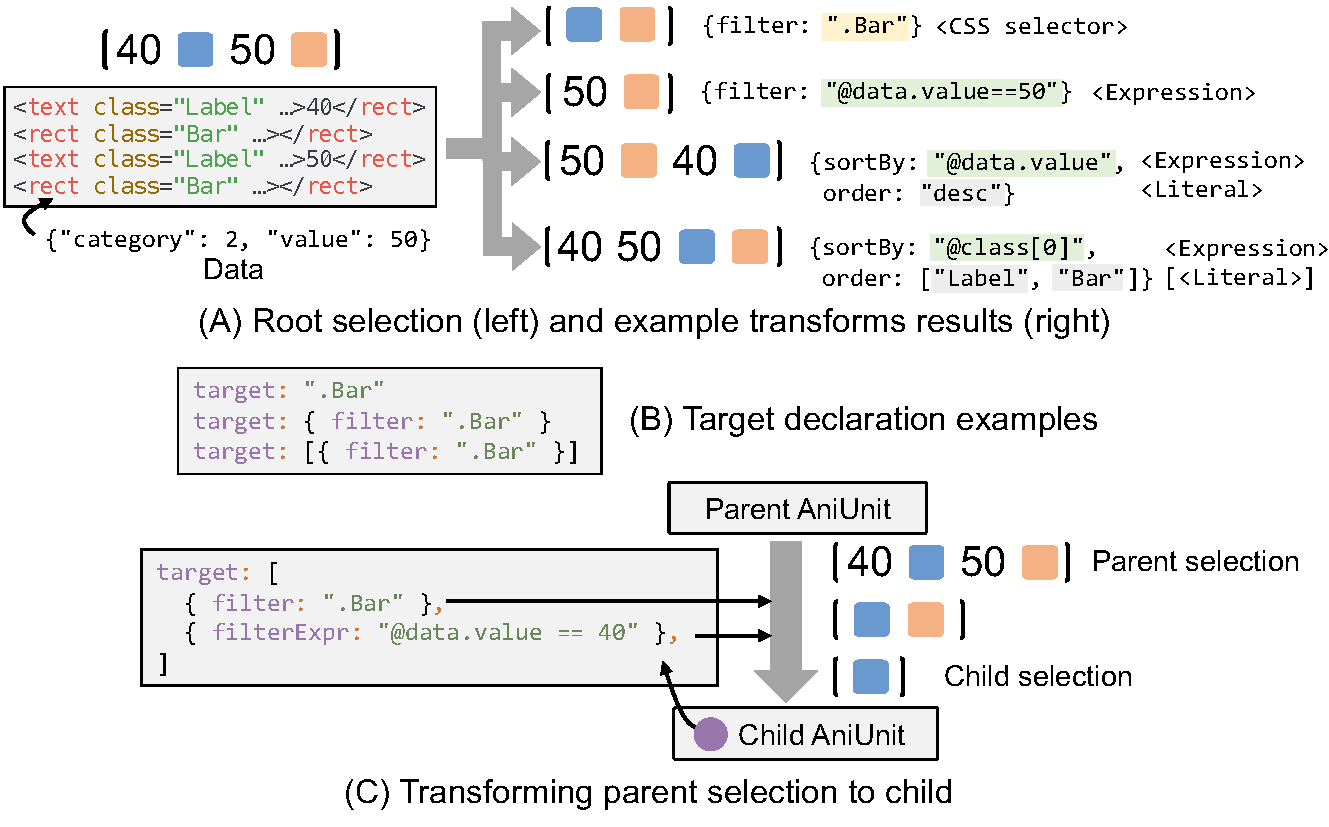
\includegraphics[width=\linewidth]{figs/transform.pdf}
  \caption{
  (A) The root selection of the SVG animated in \autoref{fig:ani_spec}. 
  (B) Examples of transform operations and the corresponding results.
  (C) Properties that can be visited in the expressions.
  (D) Declaring transform operators in attribute \code{target}.
  (E) An example of transforming parent selection to child selection.
  }
%  \Description{
%    (A) The root selection of the SVG animated in \autoref{fig:ani_spec}. 
%    (B) Examples of transform operations and the corresponding results.
%    (C) Properties that can be visited in the expressions.
%    (D) Declaring transform operators in attribute \code{target}.
%    (E) An example of transforming parent selection to child selection.
%  }
  \label{fig:target}
\end{figure}

% Attribute \code{target}, to be specific, declares how to generate target selection from its parent's selection via a sequence of \textit{transform}s.
% We denote the result of transformations as \textit{selection}, which is defined as a collection of groups.
% Intuitively, the selection representing the entire instance (called the root selection) is a collection containing the root group (as shown in \autoref{fig:target}(C)).
% \gaia{} offers four basic types of transform operators, enabling the transformation of one selection into another (\autoref{fig:target}(D-G)):

Attribute \code{target}, to be specific, declares how to generate target selection from its parent's selection via a sequence of \textit{transform}s.
Transform operators in the target attribute are concatenated, working like a pipeline between the parent and child \aniunit{}, allowing users to customize it according to their needs.


\gaia{} offers several basic transform operators, enabling the transformation of one selection into another:

\squishlist

\item \textbf{Filtering}
eliminates all unmatched elements in the collection using either a CSS selector or a predicate expression (two examples are shown in \autoref{fig:target}(B)).

\item \textbf{Sorting}
reorders elements in the collection based on a key expression (two examples are shown in \autoref{fig:target}(B)).
The desired order can be specified using keywords \code{asc} or \code{desc} (only for numerical keys) or by providing a custom list.

\item \textbf{Selecting}
functions similarly to the select and selectAll operator in D3 \cite{bostock2011d3}, querying the descendants within one or multiple groups with a CSS selector.
It allows \gaia{} to process \code{<g>} elements.
%The queries are related to target type structure introduced in \autoref{sec:gaia_reuse}.

% \item \textbf{Grouping}
% organizes groups/elements in the collection into new groups based on a specified key derived from the given expression.

\squishend

Other valid transforms include \textbf{Slicing} (extracting a portion by specifying a start, end, and step) and \textbf{Picking} (selecting one element using index).
The expression will be evaluated during the compilation.
When using expressions, \gaia{} allows users to visit several properties of elements via alias started with symbol \code{@}.
\autoref{fig:target}(C) gives a full list of supported properties.
% In fact, the selection is not performed on the real structure of SVG.
% \gaia{} provides an abstraction layer as introduced in \autoref{sec:gaia_reuse}.

\subsection{Timing}
\label{ssec:gaia_ani_timing}

As listed in \autoref{fig:ani_spec}(C), Timing encompasses 5 attributes: duration, offset, yoyo, stagger, and start.
These attributes govern the timing settings of an \aniunit{}.
Offset is used by the parent animation (\eg sync or concat) to introduce a time delay.
Yoyo enables the implementation of emphasizing animations (\eg blink, highlight, \etcns) by specifying the number of repeats and the delay between each repetition.
Stagger creates animations for each element in the list with an offset compared to the previous one, significantly simplifying "domino effects" as highlighted in \cite{shi2021communicating}.
It can be passed to some basic effect (\eg Wipe) or used with \code{foreach}.
Similar to Canis \cite{ge2020canis}, \code{start} control the reference for staggering in \code{foreach} animation, which can be \code{"with prev"} (start with previous) or \code{"after prev"} (start after previous).

One key consideration for \gaia{}, unlike other techniques, is the application of timing settings (\ie duration) within nested \aniunit{}s.
In \gaia{}, each animation has 4 timing settings: 
(1) inheritance from its parent (\eg a sync animation with a specified duration), 
(2) its own individual settings, 
(3) settings computed from its children (\eg a sync animation consisting of several child animations with set durations) and 
(4) default settings.
\gaia{} prioritizes non-null timing settings in order, and in case of conflicts, it rescales current animations or their children to resolve the conflicts.


\subsection{Effect and Parameters}
\label{ssec:gaia_ani_effect}

Attributes of type \textit{Effect} include all effect-related settings.
In fact, all animation effects can be specified by an animation type identifier along with a set of animation parameters.
For instance, in \autoref{fig:ani_spec}(A), the Wipe animation (lines 7-12) is invoked using the value of \code{ref} with \code{from} serving as the parameter passed to it. 
The parameters can be strings, numbers, boolean, and \aniunit{}s, which provides a flexible way to customize the animation.
For string or number params, users can also use them as a part of other string values, which is useful when defining CSS selectors or expressions to process targets.
As we mentioned above, params can also be used as local variables to prevent declaring several same pieces of spec.
These \aniunit{}s, which include a \code{ref} field, act as the leaf nodes in the animation spec. 
\gaia{} offers a library containing 20+ common animations for different types of elements, such as Fade, Wheel, PathDraw, and more. 
What's more, users can register their own animations in the library and reuse them as needed. 
The library and reusability are the core of \gaia{}, as elaborated further in \autoref{sec:gaia_reuse}.

\begin{figure}[h]
  \centering
  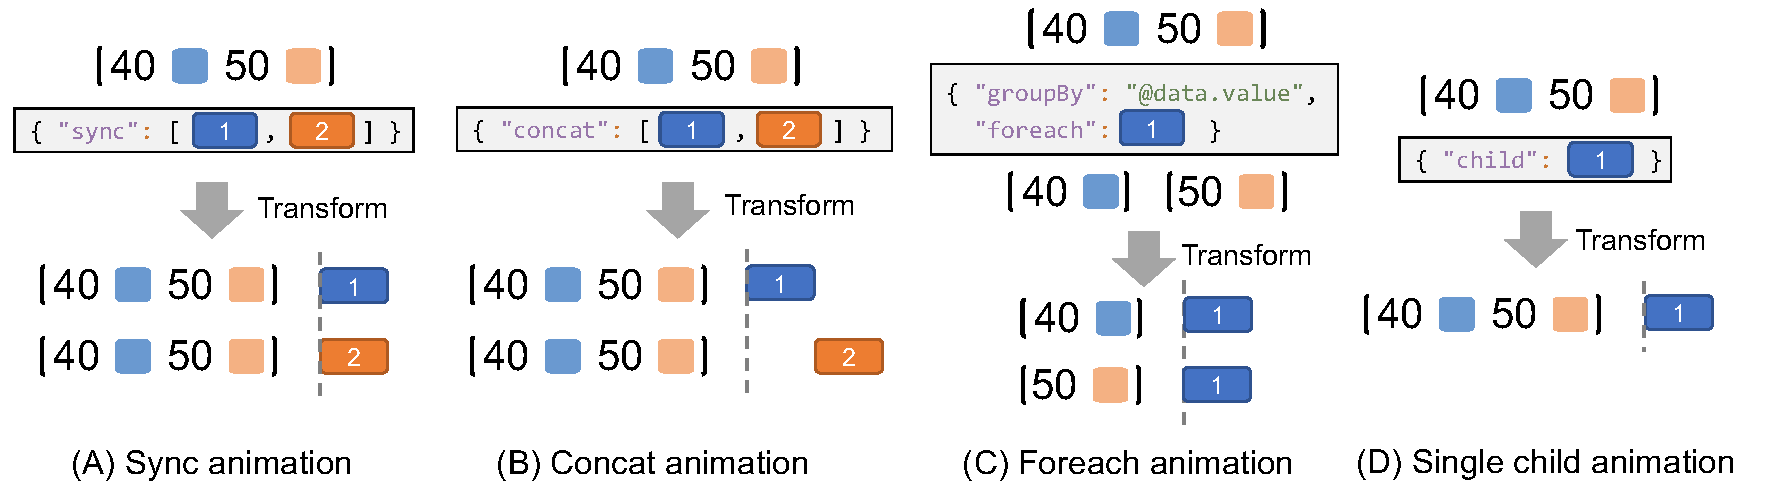
\includegraphics[width=0.9\linewidth]{figs/ani_unit_type.pdf}
  \caption{
    Examples for non-leaf \aniunit{}s (sync, concat, foreach, single-child) in \gaia{}.
  }
%  \Description{Examples for non-leaf \aniunit{}s (sync, concat, foreach, single-child) in \gaia{}.}
  \label{fig:ani_unit_type}
\end{figure}

For non-leaf \aniunit{}s, \eg sync or concat, the children can be treated as one of the parameters as well.
\autoref{fig:ani_unit_type} shows such \aniunit{}s in \gaia{}.
In sync animation, all children are aligned to the start time of this animation.
Concat animation, on the other hand, provides an alternative for building animation hierarchies, where the start time of each child is the end time of the previous one.
In both cases, the \code{"offset"} value defined in the children can further refine the declaration.
In the foreach animation, the elements in the parent selection are first grouped by the value computed by \code{"groupBy"}, and then \gaia{} creates a child animation for each group.
The single-child animation will simply apply the effect on its selection.
It is useful when the inner animation is defined as a parameter.
Except for the foreach animation, all other animations pass the parent selection to the child animation directly with transforming.

\section{Reusability and Extensibility}
\label{sec:gaia_reuse}

%As mentioned earlier, reusing not only accelerates the design process for beginners but also eases the design of repeated parts within a single animation.
%The central concept behind \gaia's reusability lies in decoupling animation designs from specific animated targets, drawing inspiration from the bridge pattern in OOP.
%In this section, we will delve into target type abstraction and demonstrate how our target type system operates within the animation specification.

Some infographics have similar semantic components, and animations of these components are also similar.
Reusing these animation benefits creating progress \cite{thompson2020understanding}.
However, their structures in the form of SVG differ from each other.
For example, the order of elements or hierarchy made by \code{<g>} might vary inside SVG code. 
Reusing animation across different instances requires a unified target abstraction.
In the previous section, we introduce the attribute \code{target} in animation spec, discussing how \gaia{} manages the targeted elements of each \aniunit{}.
In fact, these target specs are performed on an abstraction layer, as we call \textit{virtual target model}, instead of original SVGs.
In this section, we will discuss the target abstraction and explain how it enables reusability and extensibility of \gaia{} animation spec.

\subsection{Target Abstraction and Reusing}
\label{sec:target_type}

% We follow the intuition that the animated targets have a tree-like hierarchy, which is similar to the SVG DOM tree or the concept of scene graph \cite{satyanarayan2015reactive}.
% So the target abstraction in \gaia{} is the same as the target model introduced in \autoref{ssec:gaia_ani_target}, which is a tree-like structure formed by groups.
% The difference is that for each group node in the target abstraction, we assign a type to it, which is called target type.
% Each type of animated target, defined by target type spec (introduced in \autoref{ssec:target_type_decl}), has a set of declared components, which represents the types of its children.
% Then a concrete \textit{target type tree} can be created (\autoref{fig:virtual_target_model}(A)), which further defines the backbone of the virtual target model.
% Original SVG elements are appended to corresponding nodes in the virtual target model.
% \autoref{fig:virtual_target_model}(B) shows an example for the animated infographic and its SVG in \autoref{fig:virtual_target_model}(C).
% One of the advantages of this design is that users can still use id/class on the original elements to select animation targets~\footnote{Design of the virtual target model can be in other forms and replaced in our implementation smoothly.}.
% From the point of view of the original SVG, the virtual target model is a kind of reformatting.
% This process is done by another JSON spec named binder (\autoref{ssec:binder_spec}). 

The virtual target model employs the same target selection mechanism in \autoref{ssec:gaia_ani_target}.
However, in the virtual target model, elements in the list of target selection are not the original SVG elements.
To provide sufficient abstraction capability, the design of the virtual target model should be carefully considered.
We found that the animated targets have a tree hierarchy, which is similar to the SVG DOM tree or the concept of scene graph \cite{satyanarayan2015reactive}.
According to the insights from Kim \etal~\cite{kim2020gemini}, users might specific sub-elements like \textit{the x-axis title}.
Motivated by these findings, we design the target abstraction as a tree-like structure to support such expressions. 
Specifically, the target abstraction is a tree shown on the left side of \autoref{fig:virtual_target_model}, as we call \textit{target type tree}.

\begin{figure}[h]
  \centering
  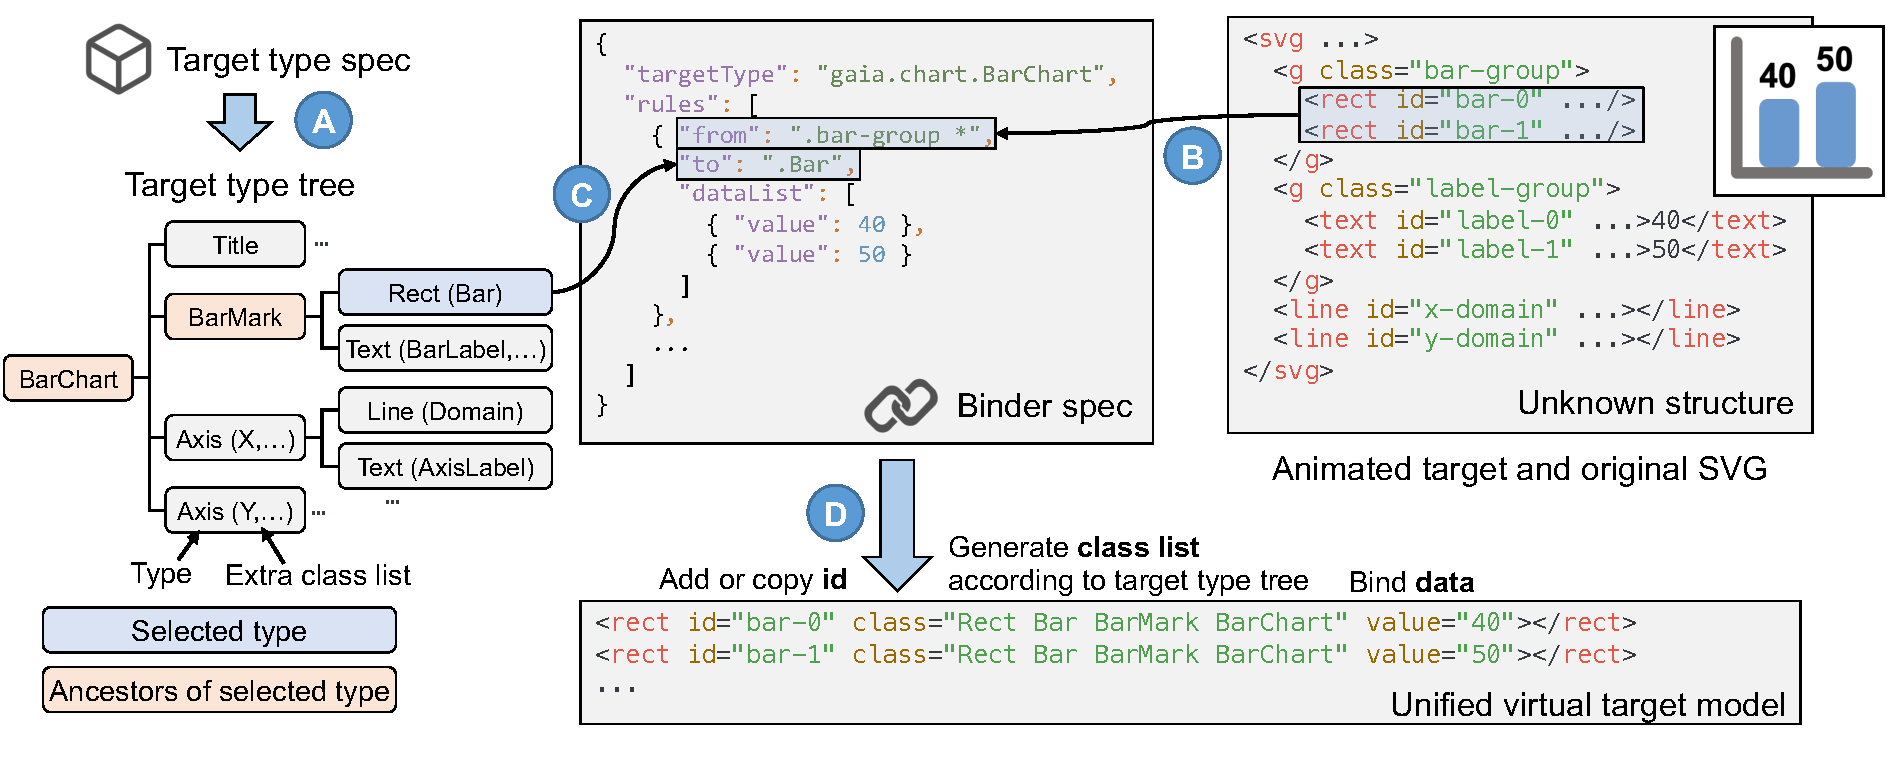
\includegraphics[width=\linewidth]{figs/target_workflow.pdf}
  \caption{Steps to create a virtual target model, which can be used as a unified representation of a class of infographics.}
%  \Description{Steps to create a virtual target model, which can be used as a unified representation of a class of infographics.}
  \label{fig:virtual_target_model}
\end{figure}

Target type trees are defined using a JSON-style spec, named target type spec (\autoref{fig:virtual_target_model}(A), introduced in \autoref{ssec:target_type_decl}).
Then, with a binder spec (\autoref{ssec:binder_spec}), the original SVG elements can be bound to a semantic type by linking it to a node of the target type tree (\autoref{fig:virtual_target_model}(B, C)).
Then a virtual target model can be generated (\autoref{fig:virtual_target_model}(D)), which is a list of virtual SVG elements.

With the virtual target model, all animated instances, \ie SVG, of the same type can be represented as a list of elements with class lists defined by the target type tree.
The target attributes in animation spec are applied on this virtual layer, which enables the reusability of animation spec regardless of the structure of SVGs.
The expert designers can represent and share their animation designs as \aniclass{}es and end users can simply reuse them using \code{ref} keyword.

\subsection{Target Type Spec}
\label{ssec:target_type_decl}

The target type spec, which defines the target types and their components, is also in JSON style.
Inspired by the object declaration in JSON schema \cite{json-schema-org}, the target type spec can declare other target types as its components via \code{ref} attribute.
As shown in \autoref{fig:type_spec}(A-C), the type declaration of BarChart contains components defined in other target type spec, declared a target type tree for BarChart shown in \autoref{fig:virtual_target_model}(A).
All these specs can be reused to form other target types, such as LineChart or Timeline.
\gaia{} manages these target types via packages and provides a set of target types for common infographics and their components.

\begin{figure}[h]
  \centering
  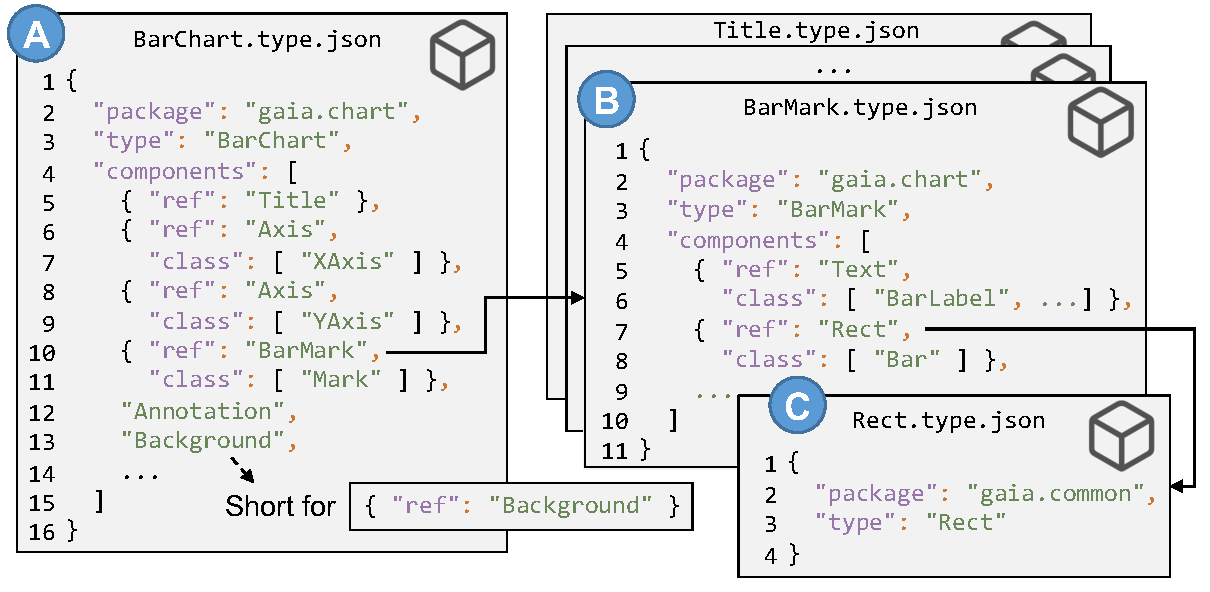
\includegraphics[width=\linewidth]{figs/target_type_spec.pdf}
  \caption{Target type can be declared using target type specs (A-C) with a specified type name and components. (D) lists the attributes used in target type spec.}
%  \Description{Target type can be declared using target type specs (A-C) with a specified type name and components. (D) lists the attributes used in target type spec.}
  \label{fig:type_spec}
\end{figure}

\autoref{fig:type_spec}(D) gives a detailed explanation of attributes in target type spec.
Notice that \code{package} can be used to avoid name conflicts.
In this case, these specs are in the same package so no import is needed (common types don't need to import).
The name of the type and class list declared in components will be used in the class list of nodes in the target type tree.


\subsection{Binder Spec}
\label{ssec:binder_spec}

Binder spec is used to bind the original SVG elements to the target type tree, and then generate the virtual target model.
As shown in \autoref{fig:virtual_target_model}, a binder spec contains attributes \code{targetType} and \code{rules}.
The value of \code{targetType} determines the target type tree to use.
Each rule in the \code{rules} (1) selects a set of elements in the original SVG by a CSS selector in \code{from}, (2) selects exactly one node in the target type tree by a CSS selector in \code{to}, and (3) binds the data to each element one by one according to the \code{dataList} attribute.
Element id can also be set if needed. 
The result is called virtual target model, which is a list of transformed SVG elements.
Each element has (1) id (\gaia{} will generate one automatically if no id is available), (2) a list of class names that come from the selected type node and its ancestors, and (3) data written to the attributes of the element.
This list will be the root selection of the animation spec, and the \code{target} of the \aniunit{} at \code{main} will be applied to it.


\subsection{Using Animation Spec as Template}
\label{ssec:extend_template}

One \aniclass{}, introduced in \autoref{ssec:aniclass_aniunit}, can be directly stored as a template and reused in other animation specs or further be a part of another template.
Notice that \aniclass{} can be declared without any concrete instance because the target is declared according to the virtual target model.
Now taking the animation in \autoref{fig:ani_hierarchy} as an example, we discuss how \aniclass{}es in \gaia{} cooperate to represent a complex animation.
Notice that end users, only need to specify the top \aniclass{} for customizability, where they can freely reuse animations from expert designers, so the progress is accelerated greatly.

\begin{figure}[h]
  \centering
  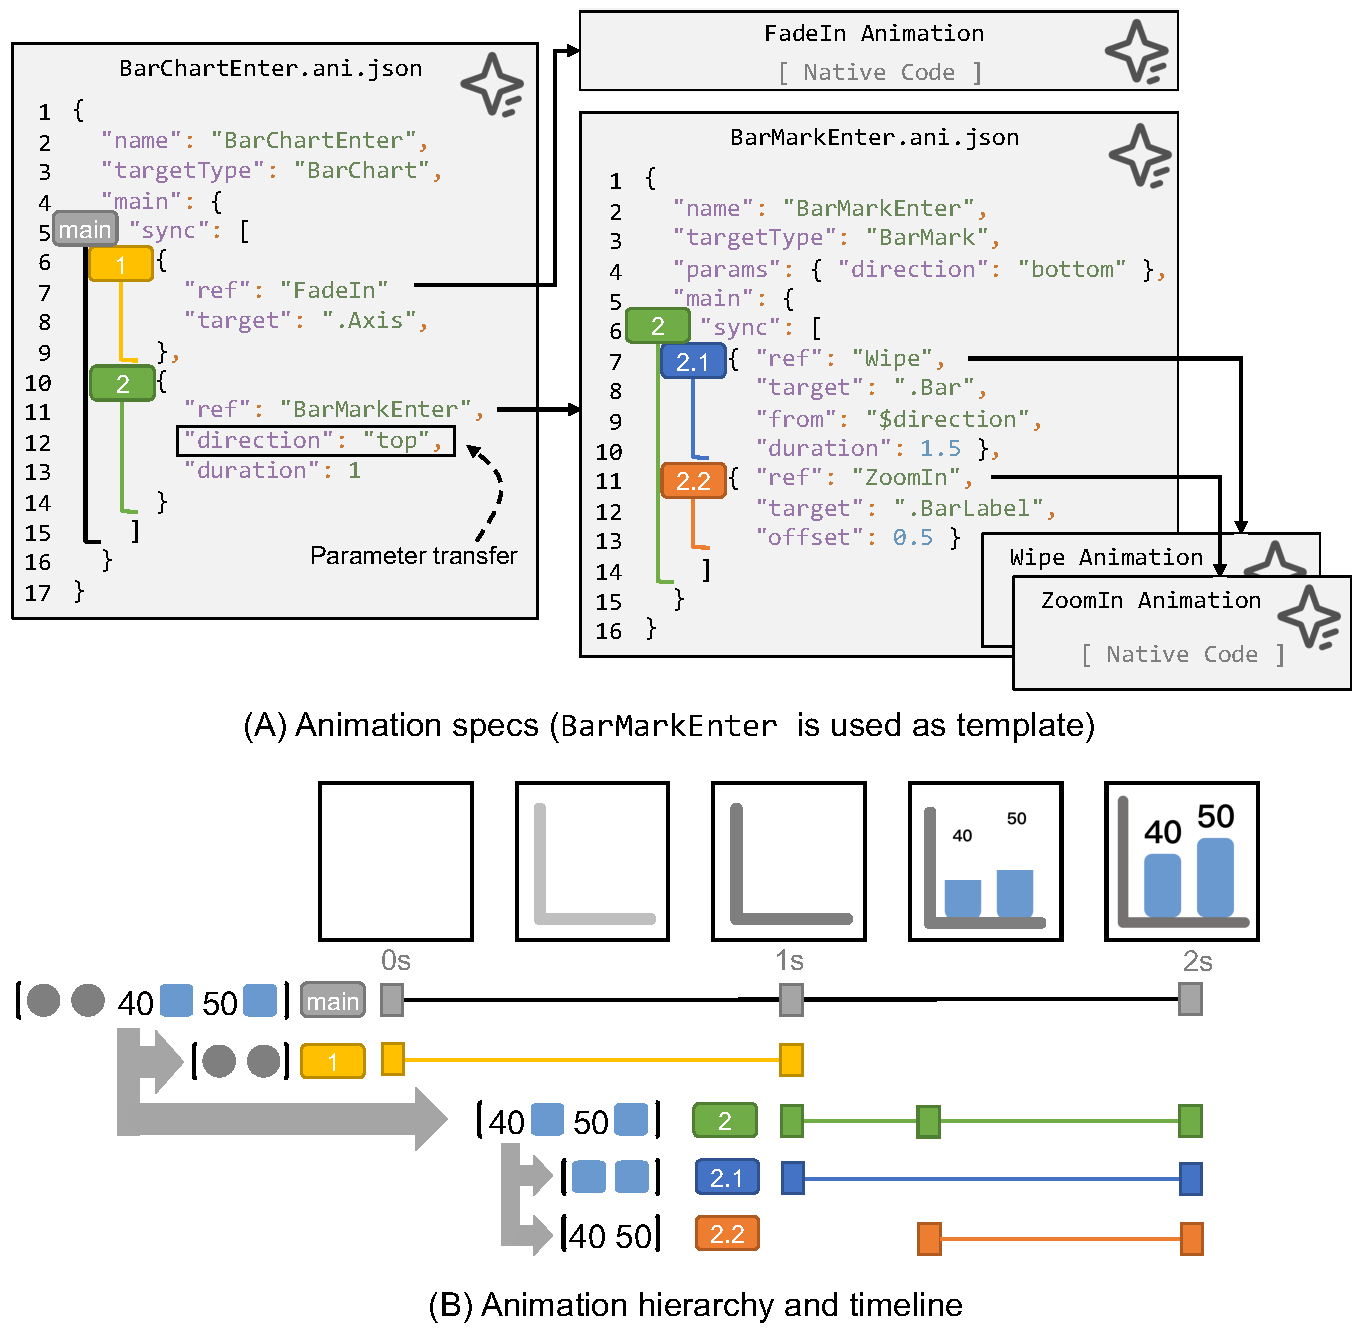
\includegraphics[width=\linewidth]{figs/ani_hierarchy.pdf}
  \caption{An example of using animation spec as a template to declare and instantiate a complex animation.}
%  \Description{An example of using animation spec as a template to declare and instantiate a complex animation.}
  \label{fig:ani_hierarchy}
\end{figure}

\autoref{fig:ani_hierarchy}(A) shows an \aniclass{} designed for BarChart. 
It refers to two sub-\aniclass{}es, FadeIn on axis components and BarMarkEnter (as same as the spec in \autoref{fig:ani_spec}(A)).
The BarMarkEnter further refers to other \aniclass{}es stored in the library, though form an animation hierarchy.
In this case, the animation spec BarMarkEnter declared using JSON is composited as a sub-animation.
It picks targets from the outer scope and the timing settings are dominated as well (rescaling duration if needed).
Parameters set in the outer scope will be transferred to the sub-animation.
Applying an SVG example, the final timeline and selected elements for each declared \aniunit{}s are shown in \autoref{fig:ani_hierarchy}(B).

Attributes of \textit{Class} specify more information of one \aniclass{}. 
Attribute \code{import} specifies other \aniclass{}s used by \code{ref} keyword, which prevents name conflicts (common \aniunit{}s don't need to import). 
\aniclass{} \code{name} is used when other \aniclass{}s refer to and reuse it (\code{"Main"} as default).
The target type that this \aniclass{} associates with is declared by \code{targetType}.
Attribute \code{params} allow users to set the parameters passed in when reusing, leaving the customizability of \aniclass{}s.
An example is shown in line 12 in \autoref{fig:ani_hierarchy}(A).

We want to emphasize that this mechanism does not rely on any concrete infographic instance. 
For example, in this case, users create an \aniclass{} for BarChart via combining existing designs for components, \ie axes and marks, without referring to a given bar chart SVG.
Then this \aniclass{} can also be registered to the library and used later.
All these things can be done in, but not limited to, a JSON-style spec, to implement the extensibility of \gaia{}.
Designers can share their animation designs with other users for reusing without the involvement of \gaia{}'s developers.


\section{Workflow and \gaia{} Compiler}
\label{sec:workflow}

In this section, we first put things together, introducing the workflow of \gaia{}, then discuss the implementation of a highly modular compiler of \gaia{}.

\begin{figure}[h]
  \centering
  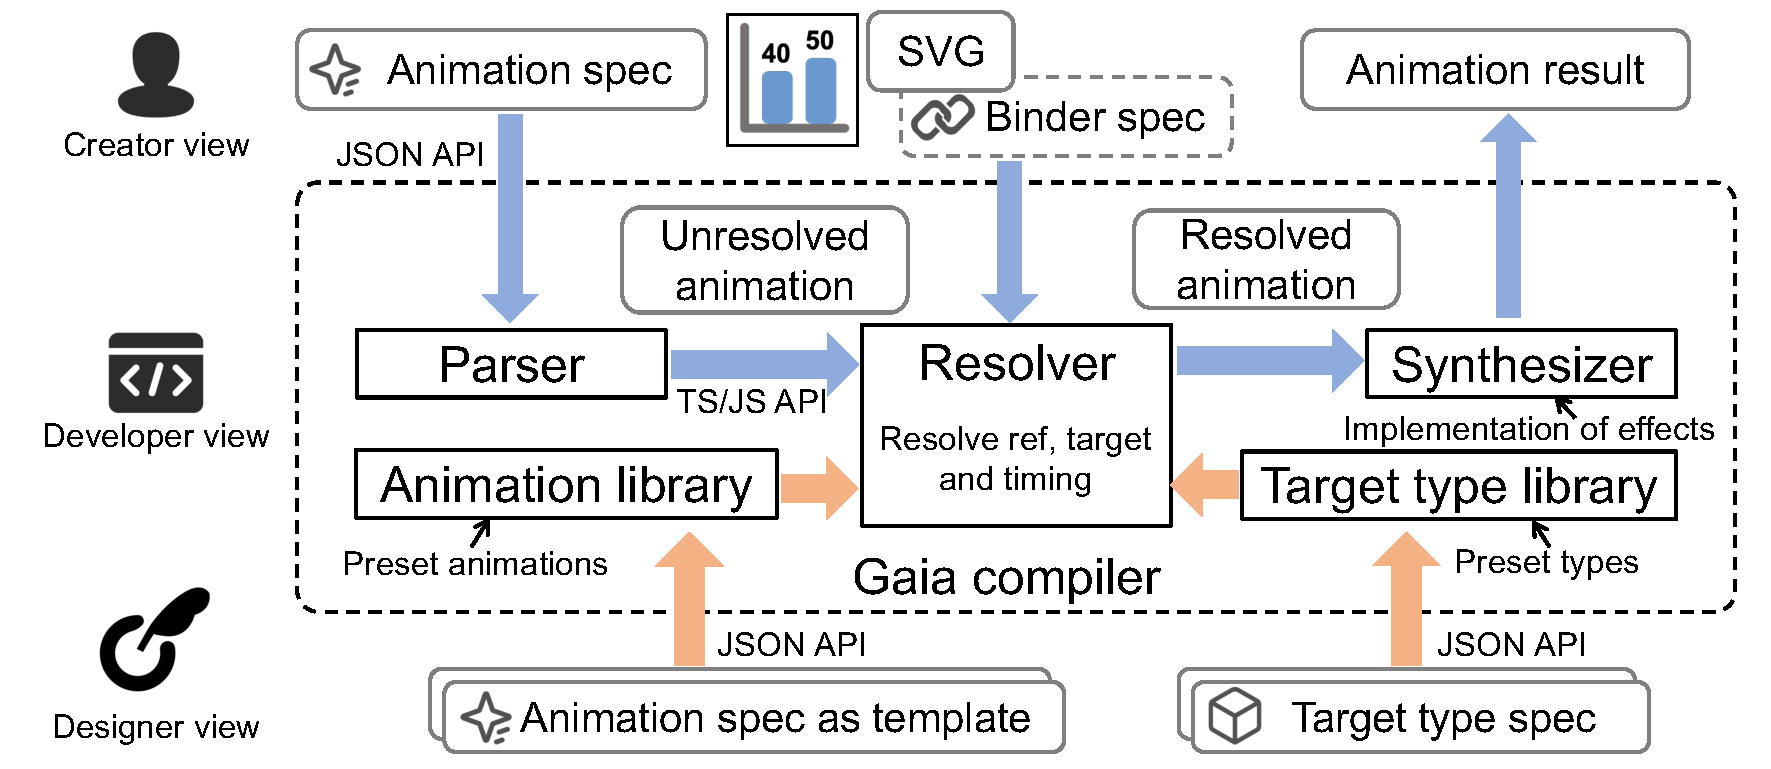
\includegraphics[width=\linewidth]{figs/workflow.pdf}
  \caption{Workflow of \gaia{} from three views and implementation of \gaia{} compiler.}
%  \Description{}
  \label{fig:workflow}
\end{figure}

\subsection{Workflow of \gaia{}}

% As shown in \autoref{fig:workflow}, the workflow is threefold:
% animations can be applied to SVGs to define animation actions

As shown in \autoref{fig:workflow}, the workflow of \gaia{} has three views.

\begin{enumerate}
\item \textbf{Creator view}.
For end users whose expectation is a visible animation, \gaia{} hides the most complexity of designing detailed animations and implementing effects. 
They only need to specify their top-level animation spec and provide an infographic with declared types. 
Creators can be human users or tools that use \gaia{} to create animations.

\item \textbf{Designer view}.
Animation design experts can design target types and provide high-quality animation templates for them.
They don't need to care about the structure of the real infographic, nor be aware of the implementation. 
Instead, they simply focus on animations from themselves or other designers using high-level grammar, creating animations that are consistent in style and mood, and clear in meaning.

\item \textbf{Developer view}.
Developers need to implement basic animation effects and serve them as code-native \aniclass{}es. In our implementation of \gaia{}'s compiler, this work is minimized as the modular design (\autoref{ssec:compiler}).
Most of the \gaia{} compiler components don't require any change when adding effects.

\end{enumerate}

The border between creators, designers and developers is not clear-cut. Creators can also build their templates and types for convenience. 
Developers can also define \aniclass{}es, like designers, with TS/JS API.
Anyway, Gaia decouples the final creator of the animation, the professional designer of the animation template and the developer of the animation effect from each other, so that each part can be developed and changed separately, and the complexity of other domains can be hidden. 
This stems from Gaia's unique reusability and extensibility.


\subsection{\gaia{} Compiler Prototype}
\label{ssec:compiler}

\gaia{} frameworks need to provide consistent, efficient APIs for different users, while ensuring reusability and extensibility at the framework level.
We implemented a prototype of \gaia{} compiler and published it as a library.
The middle part of \autoref{fig:workflow} illustrates the pipeline of the compiler.
For the creator side, the compiler takes the animation spec and the infographic as input and outputs the animation result.
The pipeline involves three steps: \textbf{parsing}, \textbf{resolving} and \textbf{synthesizing}. 
First, for any high-level spec written in JSON, a parser is used to transform it into a \gaia{} internal object using TS/JS API.
The animation spec, in this step, will form a data structure called \textbf{unresolved animation}, which is a tree-like structure.
Next, a virtual target model is created with the declared types and the given SVG.
Then, the compiler resolves the animation, linking the animations declared with \code{ref} from the library, resolving selected targets on the virtual model, and computing duration.
So far, this \textbf{resolved animation} does not rely on any specific implementation details but contains all the information for the animation.
It can be returned to the user layer for preview, debugging, or building UI (if the creator is a tool using \gaia{}).
Finally, the compiler synthesizes the resolved animation and creates the animated instance with the implementation of effects (which are tackled by developers).

It is important to note that \gaia{} provides a complete end-to-end system for creators and designers, but each component used in the compiler pipeline can be replaced.
For instance, an alternate parser can be supplied so that new features of JSON spec, or other high-level grammars, can be hired to construct unresolved animation objects.
As another example, the synthesizer can have a different implementation of the same \aniclass{} to support different element types, such as HTML and SVG, in a seamless way for high-level spec users.
Besides, the animation and target type library can be remotely stored and fetched.
We implemented a RESTful server as a remote library for internal use, which allows users to upload and download animation specs and target type specs.

\section{Evaluation}
\label{sec:eval}

In this section, we first illustrate the expressivity and reusability of \gaia{} by an animation gallery with a wide range of examples\footnote{Available in supplementary materials}. 
We conducted a user study with non-experts in animation creation, where we focused on observing the ease of use and the learning curve of \gaia{}. 
Finally, we performed semi-structured interviews with the experts who have used \gaia{} in their projects, to further understand the advantages and limitations of \gaia{}.

\subsection{Example Gallery}

\gaia{}'s expressiveness lies in two aspects: the compatibility of different kinds of infographics created by different tools and the capability to efficiently express a variety of complex animations.
Therefore, we built an animation gallery with a wide range of examples including
(1) replications of real-world data videos with different topics and styles; 
(2) generated visualizations created by Vega-Lite; and 
(3) animations of infographics adapted from related work \cite{ge2020canis,wang2021animated, cui2021mixed}.
These examples not only cover a wide range of infographic types, such as isotypes, timelines and different kinds of informative charts but also involve all animation semantic types introduced in \cite{cheng2022investigating}.
Each example includes a top-level animation spec, a set of templates used (some of them are reused from other examples), a static SVG and a corresponding binder that maps the SVG to the target type tree\footnote{For SVGs generated by Vege-Lite, binder specs can be generated automatically because the structure of SVGs is fixed.}.

As a key design goal of \gaia{}, reusability of \gaia{} enables sharing the animation design.
A lot of reuse in our gallery also simplifies the complexity of specs.
For instance, template \code{BarChartEnter} is used in the example \textit{Australia Fire}, \textit{Transportation Mode} and \textit{Wealth Inequality}.
In the example \textit{GDP Comparison} and \textit{2017 DC Courst}, template \code{ShowCategory} are invoked with different parameters, as they all include several similar entering animations for bars, bar labels, and axis labels/symbols.
To further show the reusability, we use templates to create all animations in the examples for Vega-Lite generated charts.
The template \code{ChartFrameworkEnter} is reused across the bar chart, line chart and scatter plot.
We also design generic templates used to animate series data for each different chart type with name \code{StaggeredXXXSeriesEnter}.
They animate different types of marks in a staggered way and can be reused in other charts with similar mark types.
All these templates leave the flexibility for users to customize the animation by adjusting the parameters.

Note that we also create an animation with a reusable template for a Vega-Lite bar chart without a binder, as such SVGs are generated following the same structure.
The chart is bound to the type \code{Any} so the original SVG structure can be used directly.
This case demonstrates the case without the binder, where \gaia{} can still offer the necessary support to create animations flexibly.
This feature is suggested by one of the users of \gaia{} (the first interviewee in \autoref{ssec:expert_interview}), which considers the case when users don't need the reusability supplied by the binder and virtual target model.

\subsection{User Study}
In our user study, our objective is to assess the usability of \gaia{} among novices with diverse backgrounds.
The central focus of our study revolves around the replication tasks. 
Because \gaia{}, as a descriptive language instead of an interactive creation tool, may present challenges to beginners. 
We hypothesize that even novices with no prior knowledge can use designer templates to replicate real data videos after limited learning, which is sufficient to illustrate the user-friendliness and rationality of designs like templates.

\subsubsection{Study Design}
We invited 8 participants (denoted as P1-8, aged from 22 to 28) to our user study.
All participants possess backgrounds in computer science, with P1 through P5 specializing in visualization and P2 having a background in storytelling. 
Besides, P6 also has experience in visualization.
None of them have prior experience in animation creation.

We ran the study through an online meeting one by one and each participant connected to the meeting via a desktop computer with mouse and keyboard.
They were asked to share the screen and all the interactions were recorded.
We prepared a video tutorial to introduce basic concepts about the creation of animated infographics.
Then we asked participants to complete 4 replication tasks in a web-based system\footnote{The system is the same as the demo system for case study. Materials of the user study can also be found in the demo system.}.
Before each task, we introduce the related features of \gaia{}, then provide an example to illustrate the task process.
These examples use different infographics and animations, but are implemented in the same way as in the task.

% The system is the same as the demo system for case study, with two code panels for writing \gaia{} animation/template specifications, two read-only panels for displaying binder and target models, and a preview panel for displaying animation results and timelines.
% The code panels are equipped with basic syntax highlighting.

Task 1 to 3 involve the replication of the animated infographic shown in \autoref{fig:ani_example}(a), while Task 4 entails replicating \autoref{fig:ani_example}(b).
During each task, we answered questions from participants and provided hints when they were stuck, but we avoided providing a direct answer.
We recorded the time spent on each task and the problems encountered by participants.
The details of the tasks are as follows:

\squishlist
\item \textbf{Task 1} Adjust the effect, stagger, and offset in a given animation spec to complete the replication. This task is to make sure participants understand the basic grammar of \gaia{}.
\item \textbf{Task 2} Set the target and animate each element one by one to complete the replication. Participants can understand the target abstraction and experience creating animations without involving reuse.
\item \textbf{Task 3} Create and use a template to complete the replication. We aim to let participants compare Task 2 and appreciate the benefits of reuse.
\item \textbf{Task 4} Create a new animated infographic with the template created in Task 3 and other templates provided. This task is to let participants experience the whole process of creating animations with generic templates.
\squishend

It takes about 60 minutes to watch the video and complete the task.
After finishing the tasks, we asked participants to fill out a questionnaire to collect their feedback on the primary features of \gaia{} related to each task.
We conducted a semi-structured interview as a follow-up to gain insights into their experience with \gaia{} and gather their suggestions.

\subsubsection{Results}
\label{ssec:user_study_result}

All participants could master the core features of \gaia{} in about 1 hour and use the learned abilities and provided templates to replicate the animation shown in \autoref{fig:ani_example}(b).
The average time spent on each task is about 10.63 (standard deviation SD=4.14), 6.13 (SD=2.03), 4.50 (SD=0.93), and 11.38 (SD=3.70) minutes, respectively.
The time spent on Task 1 is the largest among the first three tasks, which is mainly due to the unfamiliarity with the basic concepts of animation creation and the grammar of \gaia{}.
Some participants (3/8) struggled with the concept of offset and stagger in Task 1 so they cost more time.
After Task 2, participants are more familiar with \gaia{}, and the new concept -- templates -- is not expensive to learn, so Task 3 takes the least time and has a small standard deviation.
Task 4 contains several complex animation groups, but all of them were able to replicate within 20 minutes.

\begin{figure}[t]
    \centering
    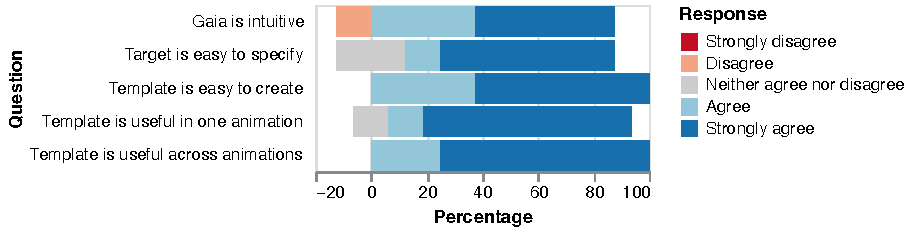
\includegraphics[width=\linewidth]{figs/user_ratings.pdf}
    \caption{User evaluations of primary features of \gaia{} using a 5-point Likert scale.}
%    \Description{User evaluations of primary features of \gaia{} using a 5-point Likert scale.}
    \label{fig:user_ratings.pdf}
\end{figure}

\autoref{fig:user_ratings.pdf} shows the results of the questionnaire.
The overall satisfaction of \gaia{} is high.
Most of the participants (7/8) think \gaia{} is intuitive and easy to use (average AVG=4.25, SD=1.04, 1 means strongly disagree and 5 means strongly agree).
P8, who gave a rank of 2, said, "\textit{I couldn't understand the stagger at first, so I got stuck.}"
However, he reported that after understanding these basic concepts, writing \gaia{} became easier.
For the target selection, most participants (6/8) took a positive attitude (AVG=4.28, SD=0.92).
The template, one of the most important features of \gaia{}, is considered to be easy to create (AVG=4.63, SD=0.52), and proves beneficial for crafting individual animated infographics (AVG=4.63, SD=0.74) as well as multiple animated infographics (AVG=4.75, SD=0.46).

In the interview, all participants agreed that \gaia{} is an easy-to-use and powerful tool for creating animated infographics.
"\textit{It let me pay more effort on design instead of effect implementation.}" P5 commented.
Participants thought that certain key features, like target selection and templates, would not incur additional learning costs.
"\textit{People who have used D3 or DOM APIs can easily get started (specifying target)}" (P1). 
Besides, some participants think the target model helps simplify the creation.
P6 told us: "\textit{target selection is a list of elements, which is more clear compared to the DOM tree.}"
Some participants mentioned that the logic of creating and using templates is similar to functions (P2, P3, P5), and the parameters can be set intuitively (P6, P7).
As for the benefits of the template, most of the participants agreed that it saves time and facilitates exploration.
P4 said, "\textit{It (template) avoids to adjust elements one by one when animations are similar but different in target/duration}".
"\textit{It is also helpful when we need to modify the animation since we only need to change the template}" (P3).

We paid attention to the mistakes participants made during the task, and tried to analyze the causes.
Setting the wrong parameters or using the wrong template are the most common mistakes.
For example, P5 tried to set the \code{from} parameters to \code{Fade} in Task 1.
\gaia{} compiler ignored the wrong parameters without any warning, causing him to start doubting whether the code had compiled successfully.
This problem was also mentioned by P1 and P7. "\textit{The system will not highlight the modified. Sometimes I wonder if the changes have taken effect}" (P1).
In addition, we also noticed that the wiping direction of the bars and lines in Task 4 is easily overlooked.
After our hints, participants still had to switch and watch the video several times before they realized the difference.

We also asked about the disappointments and improvements for \gaia{}.
More than half of the participants (P1, P2, P3, P5, P7) mentioned the lack of links between specs, SVG, and target models is a pity.
This made the debugging difficult.
"\textit{It is tedious to find useful resources in different tabs. Develop an IDE for \gaia{} might be cool}" (P3).
Besides, P3 and P6 suggested that if lambda expressions can be used to compute some values (like duration or stagger), it will be more flexible.
Three participants (P2, P3, P6) mentioned there is no gallery or document to support exploration, which is useful for novices.


\subsection{Expert Interview}
\label{ssec:expert_interview}

\gaia{} has already been used in real-world practices by several experts in the domain of animation creation and visualization. 
We kept in contact with these experts and collected their feedback during the development of \gaia{}.
In this section, we interviewed three of them (denoted as E1-3) in a semi-structured way to gather their perspectives from different views (creators and designers).
E1 has participated in some projects related to animation creation and has expertise in animation design. 
E2 is a researcher in visualization and data analysis, having experience with animation creation for more than 3 years.
The research direction of E3 is data storytelling. She has experience using animation creation tools for more than 6 years.

\subsubsection{Existing and Potential Usage Scenarios}

E1 used \gaia{}, from the view of a creator, to create videos for two months up to the time of the interview.
Both E2 and E3 use \gaia{} as the underlying animation engine to complete research work on interactive authoring and automatic generation of data videos.
They used \gaia{} for two years and one year, respectively, gaining insights into its functionality from the perspectives of creators and designers.
The work on E2 is being delivered, and the work of E3 has been published in the top conferences of visualization.
All of them think \gaia{} reduces the complexity of their tasks, simplifying the workflow and avoiding code-level implementation of motion effects.
E1 said, "\textit{\gaia{} is more powerful and customizable than other tools like PPT and can be easily integrated into our project, linking other code to the animation engine}".
E2 and E3 tried to use \gaia{} as an abstraction layer for incorporating large language models (LLMs) into the process of generating data videos.
"\textit{The most valuable aspect is that it is an abstraction layer to express, save, and reuse animations}", E2 told us.

When discussing the potential usage of \gaia{}, E1 commented that \gaia{} can support animation design in larger scenarios, not limited to 2D graphics (\eg SVG), such as VR and 3D.
Besides, E1 mentioned that \gaia{} can contribute to the adaptive UI design, such as the transition between two UI layouts.
Both E2 and E3 think that \gaia{} can benefit a wide range of users, including researchers, designers and data scientists.
"\textit{As a researcher on storytelling, I am one of the beneficiaries. In addition, \gaia{} can also help popular science video producers save time}", E3 said.

\subsubsection{Expressiveness and Learning Curve}

All of them agree that \gaia{} spec is simple and well structured, having a good balance between expressiveness and conciseness.
"\textit{All animations I need can be done via changing the parameters of templates}", E3 said.
The JSON grammar and CSS selectors make \gaia{} easy to learn and use, especially for users with a programming background (E1).
"\textit{The animations I designed are usually complex. \gaia{}'s grammar offers a controllable and predictable way to specify them.}", E1 said.
Compared to other tools like D3 and animated Vega-Lite, both E2 and E3 think \gaia{} targets a different problem and is more suitable for creating animated infographics, as other tools focus on transition and interaction, or employ a data-driven approach.

However, E1 pointed out that it is difficult for \gaia{} to express some relatively small animations, such as the blinking effect of a cat.
\textit{"My project manager thinks a large movement or stagger of multiple elements is more difficult to achieve than a small effect. But (in \gaia{}) the opposite is true" (E1)}.
E2 mentioned that when integrating \gaia{} into an automatic workflow, the parameters make things difficult.
"\textit{Some highly stylized or unusual animations are difficult to create in \gaia{}}", said E3, "\textit{they might require familiarity with \gaia{} or implementation through code.}"
Overall, though, all agreed that the ratio between the capabilities offered by \gaia{} and the cost of learning was high.

For the learning curve of \gaia{}, E1 and E3 believe that users still need to understand the JSON format and some basic knowledge in visualization and animation creation, but after that, the curve becomes very flat. 
"I tried to explain my animation design to a project manager using \gaia{}, but I find it is difficult as they even don't know the JSON" (E1).
"\textit{The difficulty of getting started depends on other experience with similar specs and background knowledge}", E3 said, "\textit{but for a programmer, this is not a problem.}"
These insights are also consistent with what we observed in the user study. 
E2 told us, "\textit{it is much easier than D3, and has a similar learning curve to animated Vega-Lite.}"

\subsubsection{Template Usage}

\gaia{} is the first high-level grammar that supports the template and supplies reusing for animations.
E1 thought the template is like functions in programming languages and can be used to encapsulate animations.
"\textit{I use templates all the time}", E1 told us, "\textit{It allows me to manage animations more clearly, even sometimes I don't reuse them.}"
In the work of E2, some complex animations are encapsulated as templates with readable names describing the effect (\eg \code{Pie-wheel-in-and-legend-fly-in}).
Then providing these animation names, element information (obtained from the target model) and narrations as prompts, LLMs can generate animations automatically.
"\textit{LLMs can understand the meaning of the animation, combine the narrative with the appropriate animation for the elements without considering the implementation details}", says E2.
E3 said that as long as a template meets the needs, she will use it first.
"\textit{They are intuitive and save time}" (E3).


\subsubsection{Extensibility}

\gaia{} allows users to create templates and extend the library in a declarative way.
E2 and E3 collaborated for an extended period.
As designers, they all craft templates according to their own needs.
E2 mentioned, "\textit{Sometimes we share the templates we have created and leave the ones we might use in our projects.}"
E2 created more than 20 templates using high-level specs, but E3 doesn't think it is necessary to create so many templates.
"\textit{Templates are most commonly used animations. A few templates will cover the needs of most cases}" (E3).

As for the consideration when designing templates, E1 thought the key point was the complexity.
"\textit{I hope the template is sufficiently generic without being overly complex to comprehend, as this would be detrimental for both myself and my collaborators}" (E1).
E2 commented the design of templates should consider the style of animated elements.
He also pointed out that some settings in a template are more likely to be changed to fit different scenarios.
As an example, he mentioned that bars might enter quickly at the beginning in some cases, but slowly in others, so letting the duration of these key elements be customizable is a good idea.

E2 also provides some insights for \gaia{} improvements. He suggested implementing effects for specific purposes.
For example, the effects used to create animations for children need to be more fun (like bar bounce).
In addition, emotional factors may also be a consideration to expand the effects.

\section{Discussion}
\label{sec:discuss}

\gaia{} is the first declarative grammar for animated infographics, which provides capabilities of flexible expression and reusability.
In this section, we discuss the design considerations, possible usages and limitations of \gaia{}.

\subsection{Cognitive Dimension}
The design of \gaia{} takes into account the Cognitive Dimension~\cite{blackwell2001cognitive}.
First, a user might act in different roles when using \gaia{} (as we mentioned in \autoref{sec:workflow}), so the consistency of the grammar is a concern.
\gaia{} uses the same grammar for both animation and template.
Consistent with the findings in the user study, this significantly reduces the cost of creating and using a template.
Besides, the tree-like spec logic for animations and target types is similar. 
Keeping some attributes consistent, such as ref, also promotes understanding.
Second, the nesting animation of \gaia{} provides a progressive learning style and supports \aniunit{} level evaluation. 
For \aniclass{} authoring, users can design a simple animation first, and then gradually add more details, each time the \aniunit{} can be evaluated immediately.
In user studies, most participants use this approach, reviewing the results as they make changes.
Third, users have the freedom to control their work steps. 
For a complex animation, users can break it down into multiple specs (\aniclass{}). 
Each spec can be evaluated individually and referred by a top-level animation so that the entire project can be completed incrementally, as stated in E1's feedback.

\subsection{Trade-off of Target Abstraction}
\gaia{} decouples the infographics creating and animation designing and employs a virtual layer for reusability.
However, users need to clarify the target type and understand the virtual model before designing animations, which might require more effort in some cases.
We determined that although the virtual layer introduces extra learning costs and usage burdens, these are outweighed by the convenience of reusing templates from professional designers, which is a relatively harder part compared to declaring the types.
In addition, virtual target models bring expert-designed animations from one instance to a class of instances, helping to express, encapsulate, and transfer domain knowledge, creating a more prosperous community environment.
As another insight, the design of the virtual target model (\eg list in \gaia{}) can be used to eliminate the complexity of real structures (as P6 said).
Finally, in the case study, we also show that \gaia{} can fall back to the original SVG structure when the virtual layer is not needed. 

\subsection{Potential Usages}
\gaia{} has the potential to be used in many more scenarios.
\gaia{} is a high-level spec that can be easily read or written directly, but it can also be used as a part of interactive tools for animated infographics authoring (E2, E3). 
Benefiting from the reusability of \gaia{}, beginners will be able to design professional animations faster and their designs can also contribute to the tools' ecosystems.
Even without exposing the reuse concept to the user, tools can take advantage of \gaia{}'s expressiveness and animation library to get the job done.
Furthermore, \gaia{} offers a well-organized format for representing both infographic instances and animations, which can obtain benefits from generative AI models. 
For instance, tools can incorporate AI to aid in animation creation with \gaia{} as an abstraction layer (E2), swiftly beginning with blank projects or carrying out design completion. 
It can even be employed to construct end-to-end generation tools for animated infographics, which is our ultimate objective and further work.
For now, the prototype of \gaia{} has already been used in some research projects for animated infographics authoring and attracted some enterprise engineers for further cooperation.

\subsection{Debugging}
Debugging declarative grammar is challenging~\cite{satyanarayan2015reactive}, and \gaia{} is no exception.
This issue is also mentioned by some participants in the user study.
With our experience working with downstream users, problems (\eg wrong syntax, empty selection and wrong parameters), will consume a lot of energy.
We implemented \gaia{} with these issues in mind, providing a complete logging system and error-handling flow. 
In addition, information related to the animation logic (such as selected elements, final animation structure, computed durations of each animation) can be obtained by the resolved animation object to facilitate debugging. 
It can also be used by developers of upper-level tools for visual animation and debugging.
Even so, we found that new users of \gaia{} still often ran into problems and struggled to get effective tips for changes. 
Smoothing the development pipeline and debugging approaches for \gaia{} is a direction worthy of further study.

\subsection{Limitation and New Opportunities}
\gaia{} introduces the target abstraction, then decouples the work for creators, designers and developers.
However, this workflow has not been fully validated.
The evaluation of expressivity is also demonstrated through the repetition of examples, rather than through the animation result implemented by professional designers.
In addition, we did not go into depth and validate the design of the target type spec and binder spec.
P5 mentioned the generalization of target types and corresponding templates can be further explored.
In expert interviews, E2 shared his experience in creating generic templates, but further research was lacking.
In addition, P5 also asked whether binder specs can be generated automatically or type binding can be done interactively.
These are the directions that can be further studied in the future.
\section{Conclusion}
\label{sec:conclusion}

In this paper, we present \gaia{}, a declarative animation grammar for animated infographics.
\gaia{} is designed to be expressive, reusable, and extensible.
We hope that \gaia{} will promote relevant academic research and practical commercial use of animated infographics.
 

\bibliographystyle{abbrv-doi-hyperref}
%\bibliographystyle{abbrv-doi-hyperref-narrow}
%\bibliographystyle{abbrv-doi}
%\bibliographystyle{abbrv-doi-narrow}

\bibliography{main}

\end{document}

